\begin{filecontents*}[overwrite]{references.bib}
@article{ramanaharan2025,
  author  = {R. Ramanaharan and D. B. Guruge and J. I. Agbinya},
  title   = {DeepFake video detection: Insights into model generalisation  A Systematic review},
  journal = {Data and Information Management},
  volume  = {9},
  pages   = {100099},
  year    = {2025}
}
@inproceedings{coccomini2022,
  author    = {D. A. Coccomini and R. Caldelli and F. Falchi and C. Gennaro and G. Amato},
  title     = {Cross-forgery analysis of vision transformers and {CNNs} for deepfake image detection},
  booktitle = {Proc. 1st Int. Workshop on Multimedia AI Against Disinformation},
  pages     = {52--58},
  year      = {2022}
}
@inproceedings{lewis2020,
  author    = {J. K. Lewis and others},
  title     = {Deepfake video detection based on spatial, spectral, and temporal inconsistencies using multimodal deep learning},
  booktitle = {IEEE Applied Imagery Pattern Recognition Workshop},
  pages     = {1--9},
  year      = {2020}
}
@article{khormali2022,
  author  = {A. Khormali and J.-S. Yuan},
  title   = {{DFDT}: An end-to-end deepfake detection framework using vision transformer},
  journal = {Applied Sciences},
  volume  = {12},
  number  = {6},
  pages   = {2953},
  year    = {2022}
}
@misc{muppalla2023,
  author = {S. Muppalla and S. Jia and S. Lyu},
  title  = {Integrating audio-visual features for multimodal deepfake detection},
  note   = {arXiv preprint arXiv:2310.03827},
  year   = {2023}
}
@inproceedings{fakeavceleb,
  author    = {H. Khalid and S. Tariq and M. Kim and S. S. Woo},
  title     = {{FakeAVCeleb}: A novel audio-video multimodal deepfake dataset},
  booktitle = {Proc. NeurIPS Datasets and Benchmarks Track},
  year      = {2021}
}
@inproceedings{lavdf,
  author    = {Z. Cai and K. Stefanov and A. Dhall and M. Hayat},
  title     = {Do you really mean that? Content driven audio-visual deepfake dataset and multimodal method for temporal forgery localization},
  booktitle = {Proc. DICTA},
  year      = {2022}
}
@inproceedings{celebdf,
  author    = {Y. Li and X. Yang and P. Sun and H. Qi and S. Lyu},
  title     = {{Celeb-DF}: A large-scale challenging dataset for {DeepFake} forensics},
  booktitle = {Proc. CVPR},
  year      = {2020}
}
@misc{dfdc,
  author = {B. Dolhansky and J. Bitton and B. Pflaum and J. Lu and R. Howes and M. Wang and C. Canton Ferrer},
  title  = {The {DeepFake} Detection Challenge ({DFDC}) dataset},
  note   = {arXiv:2006.07397},
  year   = {2020}
}
@inproceedings{ffpp,
  author    = {A. R{\"o}ssler and D. Cozzolino and L. Verdoliva and C. Riess and J. Thies and M. Nie{\ss}ner},
  title     = {{FaceForensics++}: Learning to detect manipulated facial images},
  booktitle = {Proc. ICCV},
  year      = {2019}
}
@inproceedings{syncnet,
  author    = {J. S. Chung and A. Zisserman},
  title     = {Out of time: Automated lip sync in the wild},
  booktitle = {Proc. ACCV Workshops},
  year      = {2016}
}
@inproceedings{avhubert,
  author    = {B. Shi and W.-N. Hsu and K. Lakhotia and A. Mohamed},
  title     = {Learning audio-visual speech representation by masked multimodal cluster prediction},
  booktitle = {Proc. ICLR},
  year      = {2022}
}
@inproceedings{sbi,
  author    = {K. Shiohara and T. Yamasaki},
  title     = {Detecting deepfakes with self-blended images},
  booktitle = {Proc. CVPR},
  year      = {2022}
}
@inproceedings{univfd,
  author    = {U. Ojha and Y. Li and Y. J. Lee},
  title     = {Towards universal fake image detectors that generalize across generative models},
  booktitle = {Proc. CVPR},
  year      = {2023}
}
@article{shortcut,
  author  = {R. Geirhos and J.-H. Jacobsen and C. Michaelis and R. Zemel and W. Brendel and M. Bethge and F. A. Wichmann},
  title   = {Shortcut learning in deep neural networks},
  journal = {Nature Machine Intelligence},
  volume  = {2},
  pages   = {665--673},
  year    = {2020}
}
@misc{audit,
  title = {What do deepfake benchmarks measure? An audit using frozen self-supervised representations},
  note  = {arXiv:2606.26384},
  year  = {2026}
}
@inproceedings{efficientnet,
  author    = {M. Tan and Q. V. Le},
  title     = {{EfficientNet}: Rethinking model scaling for convolutional neural networks},
  booktitle = {Proc. ICML},
  year      = {2019}
}
@article{mtcnn,
  author  = {K. Zhang and Z. Zhang and Z. Li and Y. Qiao},
  title   = {Joint face detection and alignment using multitask cascaded convolutional networks},
  journal = {IEEE Signal Process. Lett.},
  volume  = {23},
  number  = {10},
  pages   = {1499--1503},
  year    = {2016}
}
@inproceedings{wav2vec2,
  author    = {A. Baevski and Y. Zhou and A. Mohamed and M. Auli},
  title     = {wav2vec 2.0: A framework for self-supervised learning of speech representations},
  booktitle = {Proc. NeurIPS},
  year      = {2020}
}
@misc{dinov3,
  author = {O. Sim{\'e}oni and others},
  title  = { {DINOv3}},
  note   = {arXiv:2508.10104},
  year   = {2025}
}
@misc{mnw,
  author       = {{Microsoft, Northwestern University, and WITNESS}},
  title        = {{MNW} deepfake detection benchmark},
  howpublished = {\url{https://github.com/microsoft/MNW}}
}
@misc{df26,
  title        = { {DF26}},
  howpublished = {Dataset, \url{https://huggingface.co/datasets/DF26/DF26}},
  year         = {2026}
}
@book{bootstrap,
  author    = {B. Efron and R. J. Tibshirani},
  title     = {An Introduction to the Bootstrap},
  publisher = {Chapman \& Hall},
  address   = {New York},
  year      = {1993}
}
@inproceedings{convnext,
  author    = {Z. Liu and H. Mao and C.-Y. Wu and C. Feichtenhofer and T. Darrell and S. Xie},
  title     = {A {ConvNet} for the 2020s},
  booktitle = {Proc. CVPR},
  year      = {2022}
}
@article{adabn,
  author  = {Y. Li and N. Wang and J. Shi and X. Hou and J. Liu},
  title   = {Adaptive batch normalization for practical domain adaptation},
  journal = {Pattern Recognition},
  volume  = {80},
  pages   = {109--117},
  year    = {2018}
}
@misc{pe,
  author = {D. Bolya and others},
  title  = {Perception Encoder: The best visual embeddings are not at the output of the network},
  note   = {arXiv:2504.13181},
  year   = {2025}
}
@inproceedings{clip,
  author    = {A. Radford and others},
  title     = {Learning transferable visual models from natural language supervision},
  booktitle = {Proc. ICML},
  year      = {2021}
}
@inproceedings{hsemotion,
  author    = {A. V. Savchenko},
  title     = {Facial expression and attributes recognition based on multi-task learning of lightweight neural networks},
  booktitle = {Proc. IEEE SISY},
  year      = {2021}
}
@inproceedings{smeu2025,
  author    = {S. Smeu and D.-A. Boldisor and D. Oneata and E. Oneata},
  title     = {Circumventing shortcuts in audio-visual deepfake detection datasets with unsupervised learning},
  booktitle = {Proc. CVPR},
  year      = {2025}
}
@inproceedings{avff,
  author    = {T. Oorloff and others},
  title     = {{AVFF}: Audio-visual feature fusion for video deepfake detection},
  booktitle = {Proc. CVPR},
  year      = {2024}
}
@inproceedings{havic,
  author    = {J. Peng and Y. Wang and Y. Li and L. Kong and X. Hong},
  title     = {Leave no stone unturned: Uncovering holistic audio-visual intrinsic coherence for deepfake detection},
  booktitle = {Proc. CVPR Findings},
  note      = {Introduces the HAVIC detector and the {HiFi-AVDF} dataset. arXiv:2603.23960},
  year      = {2026}
}
@inproceedings{avad,
  author    = {C. Feng and Z. Chen and A. Owens},
  title     = {Self-supervised video forensics by audio-visual anomaly detection},
  booktitle = {Proc. CVPR},
  year      = {2023}
}
@inproceedings{realforensics,
  author    = {A. Haliassos and R. Mira and S. Petridis and M. Pantic},
  title     = {Leveraging real talking faces via self-supervision for robust forgery detection},
  booktitle = {Proc. CVPR},
  year      = {2022}
}
@inproceedings{lipforensics,
  author    = {A. Haliassos and K. Vougioukas and S. Petridis and M. Pantic},
  title     = {Lips don't lie: A generalisable and robust approach to face forgery detection},
  booktitle = {Proc. CVPR},
  year      = {2021}
}
@misc{speechforensics,
  author = {Y. Liang and M. Yu and G. Li and J. Jiang},
  title  = {{SpeechForensics}: Audio-visual speech representation learning for face forgery detection},
  note   = {arXiv:2508.09913},
  year   = {2025}
}
@inproceedings{zhou2021,
  author    = {Y. Zhou and S.-N. Lim},
  title     = {Joint audio-visual deepfake detection},
  booktitle = {Proc. ICCV},
  year      = {2021}
}
@inproceedings{anshul2025,
  author    = {A. Anshul and others},
  title     = {Intra-modal and cross-modal synchronization for audio-visual deepfake detection and temporal localization},
  booktitle = {Proc. ICCV},
  year      = {2025}
}
@misc{pagon2026,
  author = {S. Pagon and Y. Shen and V. Asnani and F. Liu},
  title  = {What do deepfake benchmarks measure? {An} audit using frozen self-supervised representations},
  note   = {arXiv:2606.26384},
  year   = {2026}
}
@misc{dfdlab2026,
  author = {J. Rybarczyk and M. Roszkowski and J. Komorowski},
  title  = {{DFD-Lab}: A modular audio-visual deepfake detection pipeline},
  note   = {arXiv:2609.23830},
  year   = {2026}
}
@misc{deepfakedoctor,
  author = {M. Klemt and C. Segna and A. Rohrbach},
  title  = {{DeepFake} {Doctor}: Diagnosing and treating audio-video fake detection},
  note   = {arXiv:2506.05851},
  year   = {2025}
}
@inproceedings{mueller2021,
  author    = {N. M. M{\"u}ller and F. Dieckmann and P. Czempin and R. Canals and K. B{\"o}ttinger and J. Williams},
  title     = {Speech is silver, silence is golden: What do {ASVspoof}-trained models really learn?},
  booktitle = {Proc. ASVspoof 2021 Workshop},
  year      = {2021}
}
@inproceedings{mueller2022,
  author    = {N. M. M{\"u}ller and P. Czempin and F. Dieckmann and A. Froghyar and K. B{\"o}ttinger},
  title     = {Does audio deepfake detection generalize?},
  booktitle = {Proc. Interspeech},
  year      = {2022}
}
@misc{grommelt2024,
  author = {P. Grommelt and others},
  title  = {Fake or {JPEG}? {Revealing} common biases in generated image detection datasets},
  note   = {arXiv:2403.17608},
  year   = {2024}
}
@inproceedings{dong2023,
  author    = {S. Dong and others},
  title     = {Implicit identity leakage: The stumbling block to improving deepfake detection generalization},
  booktitle = {Proc. CVPR},
  year      = {2023}
}
@misc{yu2023,
  author = {C. Yu and others},
  title  = {A unified framework for modality-agnostic deepfakes detection},
  note   = {arXiv:2307.14491. Published at ACM IH\&MMSec 2025},
  year   = {2023}
}
@inproceedings{multimodaltrace,
  author    = {M. A. Raza and K. M. Malik},
  title     = {Multimodaltrace: Deepfake detection using audiovisual representation learning},
  booktitle = {Proc. CVPR Workshops},
  year      = {2023}
}
@inproceedings{mrdf,
  author    = {H. Zou and M. Shen and Y. Hu and C. Chen and E. S. Chng and D. Rajan},
  title     = {Cross-modality and within-modality regularization for audio-visual {DeepFake} detection},
  booktitle = {Proc. ICASSP},
  year      = {2024}
}
@article{bates2023,
  author  = {S. Bates and E. Cand{\`e}s and L. Lei and Y. Romano and M. Sesia},
  title   = {Testing for outliers with conformal p-values},
  journal = {Annals of Statistics},
  volume  = {51},
  number  = {1},
  year    = {2023}
}
@article{tong2018,
  author  = {X. Tong and Y. Feng and J. J. Li},
  title   = {{Neyman-Pearson} classification algorithms and {NP} receiver operating characteristics},
  journal = {Science Advances},
  volume  = {4},
  number  = {2},
  year    = {2018}
}
@misc{nguyen2026,
  author = {D. Nguyen and others},
  title  = {When {AUC} misleads: Polarization-aware evaluation of deepfake detectors under domain shift},
  note   = {arXiv:2606.19184},
  year   = {2026}
}
@misc{laionmobile2026,
  author = {A. {von Stryk} and J. Keuper},
  title  = {{LAION-Mobile}: Evaluating deepfake detectors on one million smartphone photos},
  note   = {arXiv:2609.11134},
  year   = {2026}
}
@misc{mahdaoui2026,
  author = {M. Mahdaoui},
  title  = {How many real photos does it take? {Finite-sample} false-alarm control of frozen {AI}-image detectors under paired camera-processing shift ({Preregistration} v1.0)},
  note   = {Zenodo record 23863746},
  year   = {2026}
}
@misc{pgag2026,
  author = {S. Alqaraleh},
  title  = {{PGA-G}: Selective adaptation and conformal calibration for speech deepfake detection},
  note   = {Zenodo record 23652611},
  year   = {2026}
}
\end{filecontents*}

\documentclass[a4paper,12pt,oneside]{report}

\usepackage[
    a4paper,
    left   = 2.54cm,
    right  = 2.00cm,
    top    = 2.00cm,
    bottom = 2.50cm,
    footskip = 1.0cm
]{geometry}

\usepackage{mathptmx}
\usepackage[T1]{fontenc}
\usepackage[utf8]{inputenc}

\usepackage{setspace}
\onehalfspacing

\usepackage{xcolor}
\definecolor{Cardinal}{HTML}{B7202F}
\definecolor{CapeHoney}{HTML}{FEE1A5}
\definecolor{Eclipse}{HTML}{312016}

\usepackage{graphicx}
\graphicspath{{../figures/}}
\usepackage{tabularx}
\usepackage{booktabs}
\usepackage{array}
\usepackage{longtable}
\usepackage{multirow}
\usepackage{amsmath,amssymb}
\usepackage{caption}
\captionsetup{font=small,labelfont={bf,color=Eclipse}}

\usepackage{fancyhdr}
\usepackage{titlesec}
\usepackage[titles]{tocloft}

\usepackage{eso-pic}
\usepackage{tikz}

\usepackage[hidelinks, bookmarksnumbered]{hyperref}

% =============================================================================
% PROJECT METADATA
% =============================================================================
\newcommand{\ProjectTitle}{Shortcut-Neutral Multimodal Audio-Visual Deepfake Detection}
\newcommand{\Branch}{Electronics and Computer Engineering}
\newcommand{\BranchShort}{Electronics and Computer Engineering}
\newcommand{\Department}{Department of \BranchShort}
\newcommand{\University}{Somaiya Vidyavihar University}
\newcommand{\College}{K. J. Somaiya School of Engineering}
\newcommand{\Semester}{VII}
\newcommand{\Batch}{2023-27}
\newcommand{\AcademicYear}{2026-2027}
\newcommand{\PlaceCity}{Mumbai-77}

\newcommand{\StudentEntry}[2]{%
    \textbf{\large #1}\\[1pt]
    \normalsize Roll No: #2\\[6pt]
}

\newcommand{\GuideName}{Dr. Tejashree Phatak}
\newcommand{\GuideDesignation}{Assistant Professor}

% =============================================================================
% PAGE BORDER
% =============================================================================
\AddToShipoutPictureBG{%
    \begin{tikzpicture}[overlay,remember picture]
        \draw[Cardinal, line width=1.2pt]
            ([xshift= 1.0cm, yshift= 1.0cm]current page.south west)
            rectangle
            ([xshift=-1.0cm, yshift=-1.0cm]current page.north east);
    \end{tikzpicture}%
}

% =============================================================================
% FOOTER
% =============================================================================
\newcommand{\FooterText}{%
    \footnotesize\bfseries
    \Department\ \quad Semester \Semester\ \quad \Batch\ Batch%
}

\pagestyle{fancy}
\fancyhf{}
\renewcommand{\headrulewidth}{0pt}
\renewcommand{\footrulewidth}{1pt}
\fancyfoot[L]{\FooterText}
\fancyfoot[R]{\footnotesize\bfseries Page \thepage}

\makeatletter
\renewcommand{\footrule}{%
    {\color{Cardinal}\hrule \@height\footrulewidth \@width\headwidth}%
    \vskip-\footrulewidth%
}
\makeatother

\fancypagestyle{plain}{%
    \fancyhf{}%
    \renewcommand{\headrulewidth}{0pt}%
    \renewcommand{\footrulewidth}{1pt}%
    \fancyfoot[L]{\FooterText}%
    \fancyfoot[R]{\footnotesize\bfseries Page \thepage}%
}

\fancypagestyle{titlepg}{%
    \fancyhf{}%
    \renewcommand{\headrulewidth}{0pt}%
    \renewcommand{\footrulewidth}{0pt}%
}

% =============================================================================
% HEADINGS
% =============================================================================
\titleformat{\chapter}[display]
    {\normalfont\Huge\bfseries\color{Cardinal}}
    {\chaptertitlename\ \thechapter}{14pt}{\Huge}
\titlespacing*{\chapter}{0pt}{-20pt}{24pt}

\titleformat{\section}
    {\normalfont\Large\bfseries\color{Eclipse}}{\thesection}{1em}{}
\titleformat{\subsection}
    {\normalfont\large\bfseries\color{Eclipse}}{\thesubsection}{1em}{}
\titleformat{\subsubsection}
    {\normalfont\normalsize\bfseries\color{Eclipse}}{\thesubsubsection}{1em}{}

\renewcommand{\cfttoctitlefont}{\Huge\bfseries\color{Cardinal}}
\renewcommand{\cftloftitlefont}{\Huge\bfseries\color{Cardinal}}
\renewcommand{\cftlottitlefont}{\Huge\bfseries\color{Cardinal}}
\renewcommand{\cftchapfont}{\bfseries}
\renewcommand{\cftchappagefont}{\bfseries}
\setlength{\cftbeforechapskip}{6pt}

\setlength{\parskip}{6pt}
\setlength{\parindent}{0pt}

% =============================================================================
% BEGIN DOCUMENT
% =============================================================================
\begin{document}

% --
% TITLE PAGE
% --
\pagenumbering{roman}
\setcounter{page}{1}
\thispagestyle{titlepg}

\begin{singlespace}
\begin{center}

    \includegraphics[width=4.8cm]{1777459645157_kjsce.png}

    \vspace{8pt}
    {\Large\bfseries\color{Eclipse}\University\par}
    \vspace{2pt}
    {\large\bfseries \College\par}
    \vspace{2pt}
    {\large\bfseries \Department\par}

    \vspace{22pt}
    {\huge\bfseries\color{Cardinal} \ProjectTitle\par}

    \vspace{18pt}
    {\normalsize Submitted In Partial Fulfillment of Requirements\par}
    {\normalsize For the Degree Of\par}
    \vspace{6pt}
    {\Large\bfseries Bachelor of Technology\par}
    {\large\bfseries (\Branch)\par}

    \vspace{16pt}
    {\normalsize By\par}
    \vspace{6pt}

    \StudentEntry{Vaibhav Shiroorkar}{16014024805}
    \StudentEntry{Adithya Jithesh}{16014024803}
    \StudentEntry{Shivansh Gupta}{16014023052}


    \vspace{4pt}
    {\normalsize Guide\par}
    \vspace{2pt}
    {\Large\bfseries \GuideName \par}
    {\normalsize \GuideDesignation\par}

    \vspace{18pt}
    {\large\bfseries \University\par}
    {\normalsize Vidyavihar, Mumbai - 400 077\par}
    \vspace{4pt}
    {\large\bfseries 2026-2027\par}
\end{center}
\end{singlespace}

\clearpage

% --
% CERTIFICATE
% --
\setcounter{page}{1}

\begin{center}
    {\Large\bfseries\color{Eclipse} \University\par}
    \vspace{4pt}
    {\Large\bfseries \College\par}
    \vspace{30pt}
    {\Huge\bfseries\color{Cardinal} Certificate\par}
\end{center}

\vspace{16pt}

This is to certify that the dissertation report entitled
\textbf{``\ProjectTitle''} submitted by the following students at the end of
Semester \Semester\ of LY B.\,Tech is a bona fide record for partial
fulfillment of requirements for the degree of \textbf{Bachelor of Technology
(\Branch)} of \University.

\vspace{12pt}

\begin{tabular}{@{}p{0.5\textwidth}p{0.45\textwidth}@{}}
    \textbf{Vaibhav Shiroorkar} \quad (16014024805) & \\[8pt]
    \textbf{Adithya Jithesh} \quad (16014024803) & \\[8pt]
    \textbf{Shivansh Gupta} \quad (16014023052) & \\
\end{tabular}

\vspace{60pt}

\noindent
\begin{tabular}{@{}p{0.45\textwidth}@{\hspace{0.05\textwidth}}p{0.45\textwidth}@{}}
    \rule{6cm}{0.4pt} & \rule{6cm}{0.4pt} \\
    \textbf{Guide} & \textbf{Head of the Department} \\[2pt]
    \GuideName & Dr. Jagannath Nirmal \\[20pt]

    \rule{6cm}{0.4pt} & \rule{6cm}{0.4pt} \\
    \textbf{Examiner} & \textbf{Director} \\[2pt]
    & \\
\end{tabular}

\vspace{30pt}

\noindent\textbf{Date:}\\
\noindent\textbf{Place:} \PlaceCity

\clearpage

% --
% DECLARATION
% --
\begin{center}
    {\Large\bfseries\color{Eclipse} \University\par}
    \vspace{4pt}
    {\Large\bfseries \College\par}
    \vspace{30pt}
    {\Huge\bfseries\color{Cardinal} Declaration\par}
\end{center}

\vspace{12pt}

We declare that this written report submission represents the work done based
on our and / or others' ideas with adequately cited and referenced the
original source. We also declare that we have adhered to all principles of
intellectual property, academic honesty and integrity as we have not
misinterpreted or fabricated or falsified any idea / data / fact / source /
original work / matter in our submission.

\vspace{6pt}

We understand that any violation of the above will be cause for disciplinary
action by the college and may evoke the penal action from the sources which
have not been properly cited or from whom proper permission is not sought.

\vspace{30pt}

\renewcommand{\arraystretch}{2.4}
\begin{tabular}{|p{0.45\textwidth}|p{0.45\textwidth}|}
    \hline
    \textbf{Signature of the Student} \newline\rule{6cm}{0.4pt}\newline
    \textbf{Roll No.} \rule{4cm}{0.4pt} &
    \textbf{Signature of the Student} \newline\rule{6cm}{0.4pt}\newline
    \textbf{Roll No.} \rule{4cm}{0.4pt} \\ \hline
    \textbf{Signature of the Student} \newline\rule{6cm}{0.4pt}\newline
    \textbf{Roll No.} \rule{4cm}{0.4pt} &
    \textbf{Signature of the Student} \newline\rule{6cm}{0.4pt}\newline
    \textbf{Roll No.} \rule{4cm}{0.4pt} \\ \hline
\end{tabular}
\renewcommand{\arraystretch}{1.0}

\vspace{24pt}

\noindent\textbf{Date:}\\
\noindent\textbf{Place:} \PlaceCity

\clearpage

%
% ABSTRACT
%
\chapter*{Abstract}
\addcontentsline{toc}{chapter}{Abstract}

Audio-visual deepfake detectors report high accuracy on their own benchmarks
and fail on clips from anywhere else. This report asks how much of that
benchmark accuracy comes from how the files were made, rather than from what
they show. We audit four corpora with classifiers that see only file metadata
and the edges of the audio track. On FakeAVCeleb these cues alone predict the
real-or-fake label at an AUC of {{audit.fakeavceleb.raw.clip}}. Generated
voices are stored as MP3 where real voices are AAC. Most face swaps are
MPEG-4 Part 2 where real clips are H.264. Generated speech also carries digital
silence at its edges. LAV-DF reaches {{audit.lavdf.raw.clip}} from weak cues
combined, DFDC reaches {{audit.dfdc.raw.clip}}, and HiFi-AVDF, built with six
commercial generators, reaches {{audit.hifiavdf.raw.clip}}.

We then build a shortcut-neutral protocol. Every clip gets one codec, a fixed
3.00 s span that starts at the first sound, a fixed loudness and a low level of
dither. Our first version failed, with a ceiling of
{{audit.fakeavceleb.v1.clip}}, because re-muxing exposed hidden AAC padding.
The final version lowers the FakeAVCeleb ceiling to
{{audit.fakeavceleb.neutral.clip}}. That misses our preregistered bar of 0.60,
and we report it as a miss.

On the neutral copies we train a lip-sync detector on real clips only, on top
of frozen AV-HuBERT features. It never sees a fake. Its test AUC is
{{sync.test.seed17.auc}}, {{sync.test.seed29.auc}} and
{{sync.test.seed43.auc}} at three training seeds. Its scores follow the
mechanism it was built for: voice cloning is caught best, and face swaps that
keep the original lips and voice are caught least. Its weak point is false
alarms at a threshold carried over from validation. On LAV-DF, DFDC and
HiFi-AVDF, which it never saw, its AUC falls to between
{{sync.dfdc.seed17.auc}} and {{sync.lavdf-window.seed29.auc}}. A threshold set
from 200 real clips of the new corpus flags
{{h4.hifiavdf-seed43.conformal_real_only.fpr}} to
{{h4.hifiavdf-seed17.conformal_real_only.fpr}} of real HiFi-AVDF clips,
against {{h4.hifiavdf-seed43.source_validation.fpr}} to
{{h4.hifiavdf-seed17.source_validation.fpr}} with the threshold carried over
from training, but it then catches few fakes.

A late fusion of visual, audio and sync paths passes its preregistered test
against the visual path alone. Its gain comes from fakes the visual path cannot
see, and on LAV-DF from a visual path that ranks fakes below chance. In
exploratory checks, no fixed fusion of these paths transferred between
corpora, and stronger frozen backbones (CLIP and XLS-R) did not transfer
better on the cleaned data. All hypotheses were written
down and committed before the runs. Every result in this report is filled in
from a committed result file. A few counts that explain amendments A9 and A10
are quoted from those dated amendments.

\clearpage

%
% ACKNOWLEDGEMENTS
%
\chapter*{Acknowledgements}
\addcontentsline{toc}{chapter}{Acknowledgements}

We thank our guide, \textbf{\GuideName}, for her help throughout this project.
That help went well beyond formal reviews. When we were stuck she pointed us in
a useful direction. When it was better for us to work something out ourselves,
she gave us room to do that. This report spends many pages on our own
mistakes. Her encouragement to write openly about what failed made it a better
report than a purely positive one would have been.

We are also grateful to the faculty and staff of the \Department\ at \College\
for the resources and support behind this work. We thank the authors of
FakeAVCeleb, LAV-DF, DFDC, HiFi-AVDF and AV-HuBERT for making their data and
models available to students. Finally, thanks to our families and friends for
their patience through long preprocessing runs and late evenings.

Claude (Anthropic) assisted with implementation, analysis and documentation. All design decisions, results and claims were reviewed by the authors.

\clearpage

%
% TABLE OF CONTENTS
%
\renewcommand{\contentsname}{Contents}
\tableofcontents
\clearpage

\listoftables
\addcontentsline{toc}{chapter}{List of Tables}
\clearpage

\listoffigures
\addcontentsline{toc}{chapter}{List of Figures}
\clearpage

%
% NOMENCLATURE
%
\chapter*{Nomenclature}
\addcontentsline{toc}{chapter}{Nomenclature}

\begin{tabularx}{\textwidth}{@{}>{\raggedright\arraybackslash}p{3.8cm}X@{}}
    \toprule
    \textbf{Term} & \textbf{Meaning} \\
    \midrule
    AUC (ROC-AUC)       & Area under the receiver operating characteristic curve: the chance that a random fake scores higher than a random real clip. 0.5 is guessing and 1.0 is perfect \\
    Shortcut            & A cue that predicts the label in a dataset but is not the manipulation itself, such as the video codec \\
    Cue-only classifier & A classifier that sees only file metadata and audio-edge measurements, never a face or a voice \\
    Shortcut ceiling    & The out-of-fold AUC of a gradient-boosted model given all cues at once. A detector must beat it to show it sees the manipulation \\
    Neutralization      & Re-encoding every clip the same way, cutting it to a fixed span and fixing its loudness, so file cues carry no label \\
    Neutralizer v1, v4  & The first, failed version of our neutralizer, and the version used for every result \\
    Refusal             & A clip the neutralizer does not keep because it has less than 3.00 s of sound \\
    RVRA, RVFA, FVRA, FVFA & FakeAVCeleb categories: real or fake video (RV, FV) crossed with real or fake audio (RA, FA) \\
    Identity-disjoint split & A train, validation and test split in which no person appears in more than one partition \\
    Identity-strict subset & Test clips whose every named person belongs to the test partition only \\
    Locked test set     & A dataset that may be scored but never used to train, select or calibrate anything \\
    Preregistration     & Writing down a hypothesis, its test and its success rule, and committing it before the run \\
    Amendment           & A dated change to the preregistration, committed before the result it could affect \\
    Receipt             & A record of one evaluation: the command and the hashes of its inputs, code and outputs \\
    AV-HuBERT           & A self-supervised audio-visual speech encoder, used frozen in this work \\
    Alignment head      & The small network that scores whether a lip frame and an audio frame belong together \\
    Misfit              & The alignment head's penalty for a lip and audio pair; a clip's score is its mean misfit \\
    Balanced accuracy   & The mean of the true-positive and true-negative rates \\
    FPR, TPR            & False-positive rate (real clips flagged as fake) and true-positive rate (fakes caught) \\
    Source threshold    & The decision threshold chosen on FakeAVCeleb validation and carried to a new domain unchanged \\
    Conformal threshold & A threshold set from real clips alone so that a new real clip is flagged with probability at most $\alpha$ \\
    Umbrella threshold  & The Neyman-Pearson threshold that keeps the FPR at most $\alpha$ with probability at least $1-\delta$ \\
    $\alpha$, $\delta$, $n_{\mathrm{cal}}$ & Target false-positive rate, allowed failure probability, and the number of real calibration clips \\
    Identity bootstrap  & Resampling whole people, not clips, to get a 95\% interval \\
    Seed                & The random seed of a training run; we use 17, 29 and 43 \\
    dBFS                & Decibels relative to digital full scale \\
    CRF                 & Constant rate factor, the quality setting of the H.264 encoder \\
    \bottomrule
\end{tabularx}

\clearpage

% =============================================================================
% MAIN MATTER
% =============================================================================
\pagenumbering{arabic}
\setcounter{page}{1}

%
\chapter{Introduction}
\label{ch:introduction}

\section{The Problem}

A deepfake is a video in which the face, the voice or both have been made or
changed by a generative model. Audio-visual deepfakes are the hardest case for
a viewer. A cloned voice can be laid over a real face. A real voice can drive a
generated mouth. A face swap can keep the original speech. Detectors that read
both the picture and the sound were built to catch all of these.

On their own benchmarks these detectors report AUC values in the high 0.90s.
On clips from other sources they often fall toward chance. Our own earlier
models showed the same pattern, as Chapter~\ref{ch:history} describes. The
usual explanation is that the detector has not seen enough kinds of fakes. This
report tests a simpler one. The benchmark files may carry the label in how they
were made: which codec wrote them, how long they are, and whether the audio
starts with digital silence. A model can learn those traces instead of the
manipulation. Geirhos et al. call this shortcut learning~\cite{shortcut}.

If that explanation is right, three things follow. First, a classifier that
never looks at a face or listens to a voice should score almost as well as a
real detector. Second, a detector trained and tested on copies with those
traces removed should score lower, and the drop shows how much was shortcut.
Third, a detector that cannot learn the generator's habits, because it never
sees a fake, should still work if it reads a real signal. This report measures
all three.

\section{Objectives of This Version}

This version of the project has four objectives. Each one is a measurement
that we report whether it comes out well or badly.

\begin{enumerate}
    \item \textbf{A shortcut census.} Measure how well file metadata and audio
    edges alone predict the label on FakeAVCeleb~\cite{fakeavceleb},
    LAV-DF~\cite{lavdf}, DFDC~\cite{dfdc} and HiFi-AVDF~\cite{havic}.
    \item \textbf{A shortcut-neutral protocol.} Build copies of the data in
    which those cues carry as little label information as we can manage. Test
    the result against a bar we set before the run, and report what is left.
    \item \textbf{A lip-sync detector trained on real clips only.} Score it on
    the neutral copies, by manipulation method, and check whether its pattern
    of successes matches the mechanism it was built to read.
    \item \textbf{False-alarm control from real clips only.} Compare a
    threshold carried over from training with thresholds calibrated on real
    clips from each new domain.
\end{enumerate}

The original study plan, preregistration P-001, also includes two further
tests. One asks whether fusing visual, audio and sync paths beats the visual
path alone (H2). The other asks whether a model can say which stream was faked
across corpora (H3). H2 runs in this version, under rules fixed before any
visual or audio model existed (Chapter~\ref{ch:h2}). H3 has not run;
Chapter~\ref{ch:future} states this as a limitation and gives the plan to
finish it.

\section{Contributions}

The report makes five claims. The first four match the four objectives; the
fifth is the preregistered fusion test.

\begin{enumerate}
    \item \textbf{The census.} On FakeAVCeleb the shortcut ceiling is
    {{audit.fakeavceleb.raw.clip}}. Fake audio is MP3 where real audio is AAC.
    Most face swaps are MPEG-4 Part 2 where real clips are H.264. Generated
    speech starts and ends with digital silence. LAV-DF reaches
    {{audit.lavdf.raw.clip}} from weak cues combined. DFDC is close to clean at
    {{audit.dfdc.raw.clip}}. HiFi-AVDF reaches {{audit.hifiavdf.raw.clip}}
    from frame size, fixed clip lengths, bitrate, edge silence and sample rate.
    \item \textbf{The protocol.} One codec, a fixed 3.00 s span from the first
    sound, a fixed loudness, and dither. Naive cleaning fails
    ({{audit.fakeavceleb.v1.clip}}). Our final version lowers the ceiling to
    {{audit.fakeavceleb.neutral.clip}}. We report that residual and the clips
    that cleaning removes.
    \item \textbf{The real-only sync path.} A lip-sync detector never sees a
    fake. On neutral FakeAVCeleb it reaches a test AUC of
    {{sync.test.seed17.auc}}, {{sync.test.seed29.auc}} and
    {{sync.test.seed43.auc}} at three seeds. That is above the shortcut ceiling
    of the same copies. Its per-method scores follow the mechanism.
    \item \textbf{False-alarm control.} A threshold calibrated on real clips of
    the new domain, set against the threshold carried over from training, on
    LAV-DF and HiFi-AVDF. On HiFi-AVDF the real-only threshold flags
    {{h4.hifiavdf-seed43.conformal_real_only.fpr}} to
    {{h4.hifiavdf-seed17.conformal_real_only.fpr}} of real clips, against
    {{h4.hifiavdf-seed43.source_validation.fpr}} to
    {{h4.hifiavdf-seed17.source_validation.fpr}} with the carried-over one.
    It meets the preregistered bar on HiFi-AVDF and on LAV-DF under the file
    label in every seed. The cost is recall.
    \item \textbf{The fusion test.} Visual, audio and sync paths fused by a
    model fixed in advance, against the visual path alone, on DFDC, LAV-DF and
    the identity-strict FakeAVCeleb test. H2 holds by its preregistered rule.
    But no target shows fusion improving on fakes the visual
    path can see (Chapter~\ref{ch:h2} gives the checks).
\end{enumerate}

We do not claim a new architecture. Fusion of audio and video is not new, and
neither is training a sync model on real clips. We also do not compare our
numbers with published numbers from other protocols. Those numbers come from
data that carries the shortcuts this report measures, so the comparison would
not be fair.

\section{How This Report Is Organized}

Chapter~\ref{ch:literature} reviews audio-visual detectors, known dataset
shortcuts, prior work on predicting the faked modality, and methods for
controlling false alarms. Chapter~\ref{ch:history} gives a short and honest
account of the project's earlier phases and the mistakes that shaped this
version. Chapter~\ref{ch:audit} describes the data and the shortcut audit.
Chapter~\ref{ch:protocol} describes the shortcut-neutral protocol, including
the failed first attempt. Chapter~\ref{ch:sync} describes the real-only sync
path and its in-domain results. Chapter~\ref{ch:crosscorpus} covers the
cross-corpus tests and false-alarm control. Chapter~\ref{ch:h2} runs the
preregistered fusion test and the exploratory checks that followed it.
Chapter~\ref{ch:future} lists the
limitations and the plan for the full run, and Chapter~\ref{ch:conclusions}
closes the report. Appendix~\ref{app:repro} gives the commands to reproduce
every result.

%
\chapter{Literature Review}
\label{ch:literature}

This chapter covers four bodies of work. The first is audio-visual detectors
and how they are evaluated. The second is evidence that deepfake datasets
carry shortcuts. The third is prior work on predicting which modality was
faked. The fourth is statistical methods for holding a false-alarm rate. The
chapter ends with the gap this project fills. Numbers quoted from other papers
are left out on purpose. They come from protocols that differ from ours, and
the point of this chapter is the protocols, not the scores.

\section{Audio-Visual Deepfake Detectors}

\subsection{Supervised fusion detectors}

Most audio-visual detectors train on real and fake clips and fuse the two
modalities inside the network. Zhou and Lim built one of the first, with
separate video, audio and sync streams trained jointly~\cite{zhou2021}.
AVFF~\cite{avff} trains in two stages: self-supervised learning on real talking
faces from LRS3, then supervised fine-tuning on FakeAVCeleb. It reports high
cross-dataset AUC on KoDF and DFDC subsets. It has no official code. HAVIC,
from the authors of HiFi-AVDF~\cite{havic}, pretrains on real LRS2 clips and
fine-tunes on FakeAVCeleb. It reports high AUC on KoDF and a much lower score
on its own HiFi-AVDF set of modern commercial generators. The same paper shows
that every detector it tested drops sharply on HiFi-AVDF. Anshul et al.
learn intra-modal and cross-modal synchronization on real videos before
training a detector~\cite{anshul2025}.

These papers share one protocol choice. Almost all of them train on a random
70/30 split of FakeAVCeleb that goes back to earlier work. None of the papers
we read uses a split that keeps each person on one side. FakeAVCeleb has only
about {{audit.fakeavceleb.raw.census.RealVideo-RealAudio.clips|int}} real
videos, so a random split almost certainly puts the same people in training
and test. None of these supervised detectors reports results with the
leading-silence cue removed.

\subsection{Detectors trained on real clips only}

A second family never trains on fakes. AVAD~\cite{avad} learns audio-visual
synchronization on real clips and flags clips whose sync looks unusual.
SpeechForensics~\cite{speechforensics} uses audio-visual speech
representations learned from real speech. AVH-Align~\cite{smeu2025} trains an
alignment model on AV-HuBERT~\cite{avhubert} features of real clips only. It
is the closest design to our sync path. Its authors show that their real-only
model loses almost nothing when the leading silence is trimmed, while a
supervised variant of the same model loses a lot. That result is the main
reason we chose a real-only sync path.

Older visual baselines follow the same idea in a single modality.
LipForensics~\cite{lipforensics} learns mouth movement from lip reading.
RealForensics~\cite{realforensics} uses real talking faces as self-supervision.
SyncNet~\cite{syncnet} first showed that lip and audio embeddings can be
compared directly to measure sync.

\subsection{What these papers have in common}

Reproducible baselines with official code and weights exist for AVH-Align,
HAVIC, RealForensics, LipForensics, AVAD and SpeechForensics. We have not run
any of them on our protocol yet. Chapter~\ref{ch:future} lists this as a
limitation. A fair comparison needs the baseline run on the same neutral data,
not a number quoted from its paper.

\section{Dataset Shortcuts}

\subsection{Silence in audio-visual datasets}

Smeu et al.~\cite{smeu2025} found that fake clips in FakeAVCeleb and
AV-Deepfake1M start with a short stretch of digital silence. Real clips start
with room noise. A classifier given only that silence separates real
from fake almost perfectly on both datasets. When the silence is trimmed at
test time, several supervised detectors lose much of their accuracy. The same
paper notes a trailing-silence cue on FakeAVCeleb and a weaker one on LAV-DF.
It reports no such cue on DFDC. Their fix trims silence at test time only. It
measures reliance on the cue. It does not train a model free of it.

DeepFake Doctor~\cite{deepfakedoctor} confirmed the leading-silence cue in
every FakeAVCeleb manipulation that uses fake audio. It also found the cue in
DeepSpeak v1. It showed that random temporal jitter of the input window
removes most of the reliance. It also found that FakeAVCeleb's original
leave-one-method-out protocol leaks Wav2Lip content between training and test,
and it proposed an identity split and method-family splits instead.

Pagon et al.~\cite{pagon2026} ask what deepfake benchmarks measure. A linear
probe on frozen self-supervised features comes close to bespoke detectors on
video, image and audio benchmarks. They audit no audio-visual corpus and no
file cues. DFD-Lab~\cite{dfdlab2026} trains three audio-visual detectors on
FakeAVCeleb and reports AUROC near 0.5 on a filtered Deepfake-Eval-2024
subset, with no shortcut control. Both point the same way as our results.

\subsection{Silence in speech anti-spoofing}

The same failure appeared in speech anti-spoofing years earlier. M\"uller et
al.~\cite{mueller2021} showed that genuine ASVspoof 2019 LA recordings carry
longer silences than spoofed ones. A network given only the length of the
leading silence performed far above chance. Trimming silence made strong
anti-spoofing models much worse. Their follow-up~\cite{mueller2022} showed
that models trained on ASVspoof fail on real-world recordings. The
audio-visual community did not import their fix. This project's own earlier
audio model hit the same problem (Chapter~\ref{ch:history}).

\subsection{Format and identity shortcuts}

In generated images, JPEG compression and image size differ between real and
fake sets. Grommelt et al.~\cite{grommelt2024} showed that detectors learn
those differences, and that removing them improves transfer. FaceForensics++
avoids a codec gap by compressing real and fake videos with the same
settings~\cite{ffpp}. We found no paper that publishes a per-class codec census
for an audio-visual deepfake dataset, or a classifier trained on file metadata
alone.

Dong et al.~\cite{dong2023} showed that face-swap detectors learn identity, and
that this hurts generalization. No paper we read measures identity leakage in
audio-visual detectors. A related open question is speaker overlap between a
pretrained encoder and the test data. AV-HuBERT was pretrained on LRS3 and
VoxCeleb2, and FakeAVCeleb draws on the same kinds of sources.

\section{Predicting Which Modality Was Faked}

Several papers train heads that predict the audio and video labels
separately. Multimodaltrace~\cite{multimodaltrace} uses one output per
modality on FakeAVCeleb. Yu et al.~\cite{yu2023} train a dual-label classifier
on FakeAVCeleb, DFDC and LAV-DF. They report per-modality accuracy across
datasets, between DFDC and FakeAVCeleb only, and audio accuracy collapses in
that transfer. MRDF~\cite{mrdf} argues that clip-level labels harm fused
learning, because a unimodal feature is pushed toward a label that belongs to
the other modality. Its evidence is in-dataset only.

No paper we found reports transfer of modality prediction between FakeAVCeleb
and LAV-DF, or does it under shortcut control. We planned this test as H3. It
has not run in this version.

\section{Controlling False Alarms}

A detector in use needs a threshold, and the threshold decides how many real
clips get flagged. Recent work shows that thresholds fail to transfer even
when AUC holds. Nguyen et al.~\cite{nguyen2026} found that the best threshold
varies widely from dataset to dataset for the same detector.
LAION-Mobile~\cite{laionmobile2026} found that thresholds fitted on older data
flag far more real smartphone photos than intended. We do not claim this
observation as ours.

The statistics to fix it are standard. Split conformal prediction sets a
threshold from the scores of real clips alone. A new real clip from the same
distribution is then flagged with probability at most $\alpha$. Bates et
al.~\cite{bates2023} give this guarantee for outlier testing with conformal
p-values. Tong et al.~\cite{tong2018} give the Neyman-Pearson umbrella
algorithm. It picks one of the real scores as the threshold. The choice keeps
the false-positive rate at most $\alpha$, with probability at least
$1-\delta$ over the calibration draw. Both methods need only real clips.

Two concurrent records do something close. Mahdaoui~\cite{mahdaoui2026}
preregistered real-photo recalibration for still-image detectors under camera
processing shift, with no results yet. PGA-G~\cite{pgag2026} sets conformal
operating points from genuine speech. We found no work that tests real-only
calibration for audio-visual video detectors across corpora.

\section{The Gap This Project Fills}

Each part of our method has precedent. Real-only sync models exist. Silence
shortcuts are documented. Conformal thresholds are textbook. What we did not
find in the literature is the combination below:

\begin{itemize}
    \item a per-class census of codec, silence, length and other file cues for
    several audio-visual datasets, with a single shortcut ceiling per corpus;
    \item neutral copies of both training and test data, with the residual
    ceiling measured and reported, including a failed first attempt;
    \item identity-disjoint FakeAVCeleb splits, with an identity-strict subset;
    \item a real-only detector evaluated on those copies, by method, against
    the shortcut ceiling of the same copies;
    \item real-only threshold calibration for audio-visual video under corpus
    shift.
\end{itemize}

The rest of this report describes that work.

%
\chapter{Project History and Lessons}
\label{ch:history}

This project began on 4 July 2026. The version in this report is its third
form. This chapter tells the story briefly, because the earlier phases explain
why the current protocol looks the way it does. The full log of every mistake
is in section 6 of the project handbook. Numbers from earlier phases are left
out here on purpose. They were measured under protocols this report replaces,
and several of them were later withdrawn.

\section{The Prototype (July to August)}

The first plan had five streams. Three were visual models (Xception,
EfficientNet and a self-supervised transformer). Two were cross-modal: a
lip-sync stream and an emotion-consistency stream. A fusion layer over their
embeddings would give the verdict. The idea was sound. A lip-sync fake changes
only the mouth, so the frames look real and the fake lives in the mismatch
between sound and face.

Three visual streams were trained by early August. They scored near perfect
on a held-out FakeAVCeleb split. Three faults sat behind those scores. The
validation and test sets had been undersampled to a fixed class ratio, so
every precision and recall sat at an artificial prevalence. The backbones were
ranked on the test split, which turned the test split into a selection set.
And no run record existed behind any number, because experiment tracking had
been planned but never built.

The prototype also found the project's most expensive problem and dismissed
it. On 28 July we noticed that FakeAVCeleb's Wav2Lip fakes are MPEG-4 Part 2
files while genuine clips are H.264. We treated it as a browser playback bug.
We reasoned that the decoders turn both codecs into the same kind of array, so
a model could not see the difference. That reasoning was wrong, and we did not
find out for three months.

\section{The Rebuild and the Root Study (August to October)}

On 24 August the project restarted from a new root commit, with evaluation as
the first concern. Splits were checked in code, and MLflow tracked every run.
All three branches (visual, audio and sync) and a fusion head were trained at
full scale in September. Several results changed how the project worked:

\begin{itemize}
    \item \textbf{Checkpoints were chosen on validation loss.} One stream kept
    an early checkpoint whose backbone was still frozen. It scored below
    chance. The fix to select on ROC-AUC was applied to some trainers and not
    others, and the gap survived into October.
    \item \textbf{Near-perfect in-domain scores collapsed elsewhere,} three
    times in all.
    \item \textbf{Only one seed was ever scored.} Three seeds were trained, but
    the evaluation script named the seed-17 checkpoint directly. When the other
    two were scored in October, seed 17 turned out to be the best of three. The
    spread across seeds was larger than the fusion effect it had been used to
    judge.
    \item \textbf{The attention mechanism was at chance.} The cross-attention
    streams logged how much attention fell near the diagonal. It stayed at
    chance in every run, even when the stream's accuracy was high. The models
    were accurate, but not for the reason their design claimed.
    \item \textbf{The visual model read the codec.} Re-encoding genuine clips
    with the codec of the largest fake category made most of them look fake.
    Training that cue away cost more on DFDC than it gained.
\end{itemize}

An audit in late October found three more faults. The fusion fold models had
chosen their epoch using labels from the holdout they were later scored on.
LAV-DF windows that started at zero had been shifted into manipulated spans by
a wrong default. Two image encoders had been fed inputs with the wrong
normalization. Every affected number was marked ``requires rerun''.

\section{The Team Project (October)}

From 24 October the three of us built a second system for the October
submission, under a stricter protocol. Each hypothesis and its pass line were
written down before the run. A test split was sealed and read once, after the
system was frozen. Three confirmatory tests carried a multiplicity correction.

The team project found the same two problems with different code and data. A
LAV-DF visual head passed its preregistered test, but it had learned whether a
video was an original or a produced copy, not whether it was fake. Within
produced videos it was at chance. And codec metadata alone separated real from
fake FakeAVCeleb video almost perfectly. The sealed FakeAVCeleb test had been
run on a corpus with a codec shortcut, so its strong score measured ranking on
that shortcut. Preregistrations had also been committed together with their
scripts, so git could not show they came first.

\section{The Audit of 13 November}

On 13 November we ran a dedicated shortcut audit on FakeAVCeleb
(Chapter~\ref{ch:audit}). File metadata and audio edges alone predicted the
labels. The same day we found other faults. The test suite had silently
stopped running after the repository was renamed. A file name in FakeAVCeleb's
metadata had been parsed as a person, so the identity-strict test contained no
RealVideo-FakeAudio clips at all. DFDC had never been locked, and it had been
used to choose two models. Decisions used a fixed threshold of 0.5 on data
where fakes far outnumber real clips.

\section{The Most Damaging Mistakes}

Table~\ref{tab:mistakes} names the five mistakes that cost the most, and what
each one cost.

\begin{table}[ht]
    \centering
    \small
    \caption{The five most damaging mistakes, from section 6 of the project handbook.}
    \label{tab:mistakes}
    \begin{tabularx}{\textwidth}{@{}>{\raggedright\arraybackslash}p{4.2cm}X@{}}
        \toprule
        \textbf{Mistake} & \textbf{What it cost} \\
        \midrule
        Mixed codecs found in July and judged harmless & Every in-domain FakeAVCeleb number from July to October partly measures the encoder. It is the reason for this version of the project. \\
        Only seed 17 scored, and it was the best draw & The reported cross-corpus baseline and fusion headline were best-of-three. The seed spread was larger than the effect being claimed. \\
        Fusion fold models chose epochs on their own holdout & Every fusion row from the root study, including its cross-corpus headline, needs a rerun. \\
        DFDC was not locked & DFDC chose a BatchNorm setting and an ensemble, so those DFDC numbers are partly in-sample. \\
        Checkpoints chosen on validation loss & One kept checkpoint scored below chance. Two stream results were withdrawn, and one shipped model was never fine-tuned. \\
        \bottomrule
    \end{tabularx}
\end{table}

\section{What We Changed Because of Them}

Each fault became a rule, so it cannot recur silently. We now select on the
metric we report. Every claim uses three seeds and reports their spread.
Cross-corpus results are the headline, not in-domain ones. Locked targets are
refused in code for training, selection and calibration. Thresholds come from
validation, with a record of the clips that chose them. Each hypothesis is
committed alone, before its run. And every result in a deliverable is filled
in from a result file, so no result can be typed by hand.

The biggest change is the first step. Before any model is trained, we now
measure what file cues alone can do. That step is the subject of the next
chapter.

%
\chapter{Data and the Shortcut Audit}
\label{ch:audit}

\section{The Corpora}

Table~\ref{tab:corpora} lists the four corpora and their roles. FakeAVCeleb is
the only training corpus. The other three are locked test sets: the code
refuses them for training, model selection and threshold choice.

\begin{table}[ht]
    \centering
    \small
    \caption{The four corpora used in this version. Audited counts are the files read by the shortcut audit.}
    \label{tab:corpora}
    \begin{tabularx}{\textwidth}{@{}l>{\raggedright\arraybackslash}Xr@{}}
        \toprule
        \textbf{Corpus} & \textbf{Role} & \textbf{Clips audited} \\
        \midrule
        FakeAVCeleb v1.2~\cite{fakeavceleb} & Training (real clips only, for the sync path), validation and in-domain test & {{audit.fakeavceleb.raw.clips|int}} \\
        LAV-DF~\cite{lavdf} & Locked cross-corpus test. The audit reads a stratified sample of files & {{audit.lavdf.raw.clips|int}} \\
        DFDC subset~\cite{dfdc} & Locked cross-corpus test & {{audit.dfdc.raw.clips|int}} \\
        HiFi-AVDF~\cite{havic} & Locked test on six commercial generators & {{audit.hifiavdf.raw.clips|int}} \\
        \bottomrule
    \end{tabularx}
\end{table}

\textbf{FakeAVCeleb} has four categories. RealVideo-RealAudio (RVRA) clips are
genuine. RealVideo-FakeAudio (RVFA) clips carry a cloned voice. FakeVideo-RealAudio
(FVRA) clips have a swapped or lip-synced face over real speech.
FakeVideo-FakeAudio (FVFA) clips change both. The manipulation methods are
FaceSwap, FSGAN, Wav2Lip, their combinations, and RTVC for voice cloning. The
corpus has about {{audit.fakeavceleb.raw.census.RealVideo-RealAudio.clips|int}}
real videos and many times more fakes.

\textbf{LAV-DF} edits a few words inside a longer real recording, in the audio,
the video or both. For the sync tests we sample it by original recording
(P-001 amendment A3). Each of 1,000 sampled originals comes with all its
edits, 3,823 files in total. Real and fake clips therefore share speaker, room
and camera.

\textbf{DFDC} is the existing {{audit.dfdc.raw.clips|int}}-clip subset used
throughout the project. It has
{{audit.dfdc.raw.census.RealVideo-RealAudio.clips|int}} real clips and
{{audit.dfdc.raw.census.FakeVideo-RealAudio.clips|int}} fakes. It has clip
labels only.

\textbf{HiFi-AVDF} pairs each of
{{audit.hifiavdf.raw.census.RealVideo-RealAudio.clips|int}} real videos with a
generated copy. The copies come from six commercial generators: Kling 2.5,
PixVerse V5, Seedance 1.0, Sora 2, Veo 3.1 and Wan 2.5. It is public. We added it as a
locked target in P-001 amendment A5.

\section{The Audit Method}

The audit asks one question: how well can a classifier predict the label if it
never sees a face or hears a voice? The script
\texttt{scripts/shortcut\_audit.py} reads each clip's file and measures 16
cues:

\begin{itemize}
    \item \textbf{Container and stream metadata:} container, video codec, pixel
    format, audio codec, whether audio exists, frame rate, width and height.
    \item \textbf{Rates and length:} duration, overall bitrate, video bitrate,
    audio bitrate and audio sample rate.
    \item \textbf{Audio edges:} the length of digital silence at the start and
    at the end of the track, with silence defined as below $-60$~dBFS, and the
    overall loudness.
\end{itemize}

It scores these cues against three labels: whether the clip is fake, whether
its video is fake, and whether its audio is fake. It reports two kinds of
number.

\textbf{Single-cue AUC.} Each cue on its own, ranked against the label. A cue
can point either way, so the script reports the larger of AUC and $1 -
\mathrm{AUC}$. That choice is made in-sample, so single-cue values are slightly
optimistic.

\textbf{Shortcut ceiling.} A gradient-boosted tree model gets all 16 cues at
once. It is trained and scored with five folds, and its AUC is out-of-fold.
The folds are grouped so that one group never sits on both sides. On
FakeAVCeleb the groups are source identities. On HiFi-AVDF each group is a
real clip and its generated copy. On LAV-DF the audit runs per file, not per
window. An earlier window-level run let one file supply both a real and a fake
window, which file cues cannot separate. That run understated the shortcut and
was deleted.

The ceiling is the bar for every detector on the same data. A detector that
scores below it has not shown that it reads anything the file does not
already give away.

\section{Results}

Table~\ref{tab:ceilings} gives the ceilings on the raw files.
Figure~\ref{fig:census} shows the raw and neutral ceilings side by side for
each corpus.

\begin{table}[ht]
    \centering
    \caption{Shortcut ceiling on raw files: out-of-fold AUC of a gradient-boosted model given only file and audio-edge cues. Higher means a worse benchmark.}
    \label{tab:ceilings}
    \begin{tabular}{lrrrr}
        \toprule
        \textbf{Corpus} & \textbf{Clips} & \textbf{Clip label} & \textbf{Video label} & \textbf{Audio label} \\
        \midrule
        FakeAVCeleb & {{audit.fakeavceleb.raw.clips|int}} & {{audit.fakeavceleb.raw.clip}} & {{audit.fakeavceleb.raw.video}} & {{audit.fakeavceleb.raw.audio}} \\
        LAV-DF      & {{audit.lavdf.raw.clips|int}} & {{audit.lavdf.raw.clip}} & {{audit.lavdf.raw.video}} & {{audit.lavdf.raw.audio}} \\
        DFDC        & {{audit.dfdc.raw.clips|int}} & {{audit.dfdc.raw.clip}} & {{audit.dfdc.raw.video}} & no audio fakes \\
        HiFi-AVDF   & {{audit.hifiavdf.raw.clips|int}} & {{audit.hifiavdf.raw.clip}} & {{audit.hifiavdf.raw.video}} & {{audit.hifiavdf.raw.audio}} \\
        \bottomrule
    \end{tabular}
\end{table}

\begin{figure}[htbp]
    \centering
    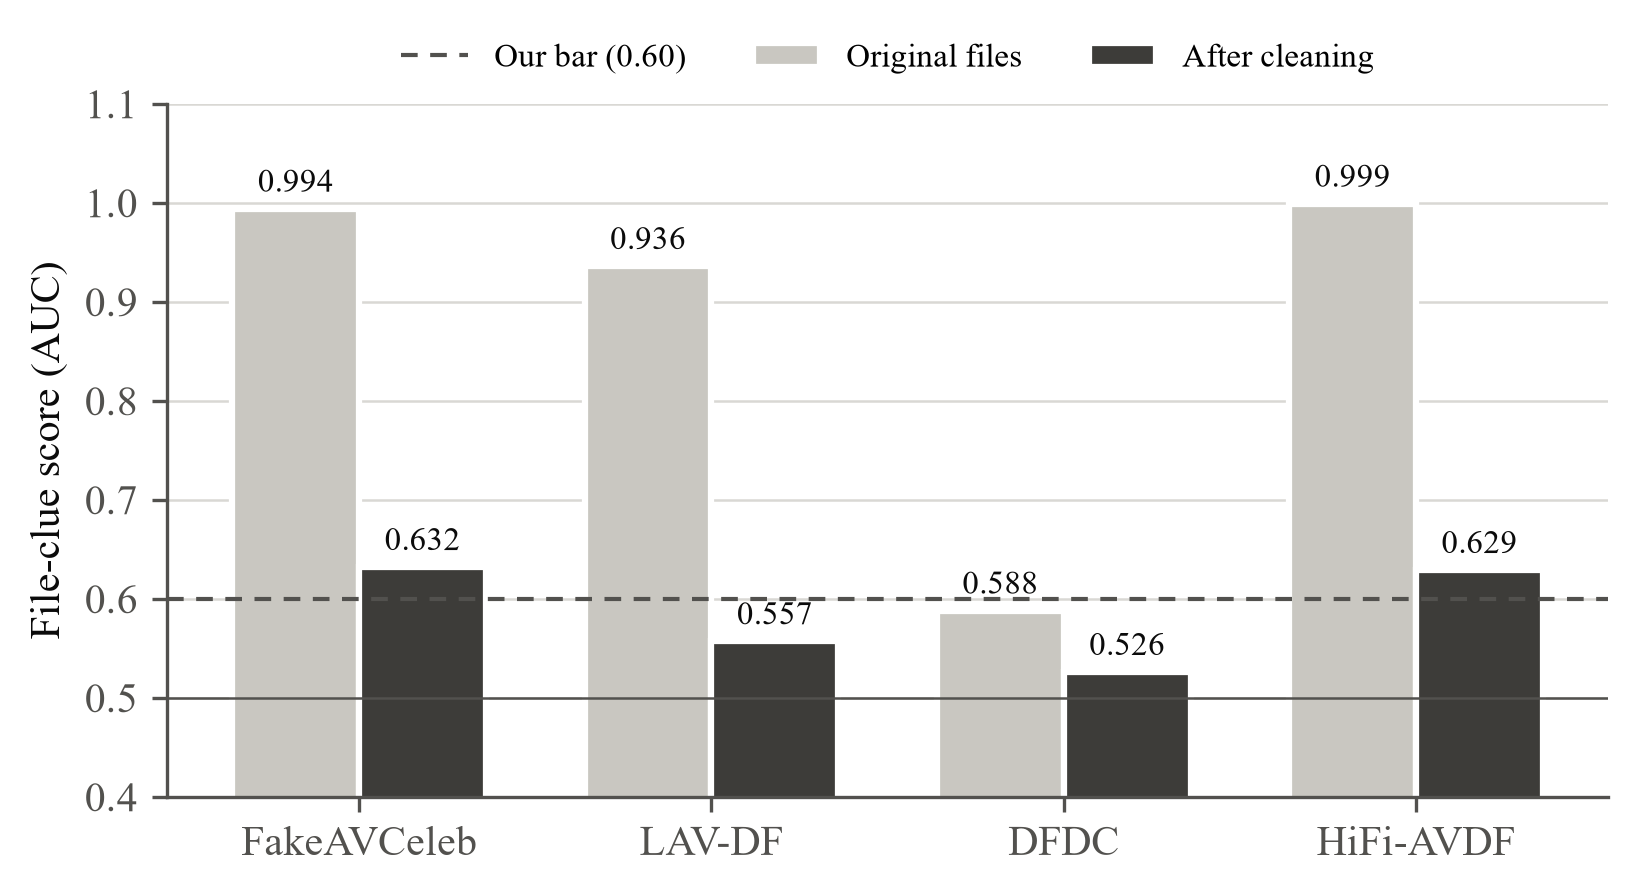
\includegraphics[width=0.85\textwidth,keepaspectratio]{fig_census.png}
    \caption{Shortcut ceiling per corpus, on raw files and on neutral copies. The dashed line marks the preregistered bar of 0.60.}
    \label{fig:census}
\end{figure}

\subsection{FakeAVCeleb}

FakeAVCeleb's labels can be read off its files. The ceiling on the clip label
is {{audit.fakeavceleb.raw.clip}}. On the audio label it is
{{audit.fakeavceleb.raw.audio}}. The strongest single cue for the clip label is
the video codec. The strongest single cue for the audio label is the length of
the leading silence.

Table~\ref{tab:census-fakeavceleb} shows why. Every real clip is H.264 video
with AAC audio. Almost every cloned-voice clip stores its audio as MP3. Most
FakeVideo-RealAudio clips, and every FakeVideo-FakeAudio clip, use MPEG-4 Part 2
video. A detector trained on these files can learn the encoder instead of the
face. Two of these cues have not been reported for this dataset before: the MP3
track on generated speech, and the per-category codec split.

\begin{table}[ht]
    \centering
    \small
    \caption{FakeAVCeleb codec census, raw files and neutral copies. Counts are clips per codec.}
    \label{tab:census-fakeavceleb}
    \begin{tabularx}{\textwidth}{@{}l r >{\raggedright\arraybackslash}X >{\raggedright\arraybackslash}X r@{}}
        \toprule
        \textbf{Category} & \textbf{Raw clips} & \textbf{Raw video codec} & \textbf{Raw audio codec} & \textbf{Neutral clips} \\
        \midrule
        RVRA & {{audit.fakeavceleb.raw.census.RealVideo-RealAudio.clips|int}} & H.264 ({{audit.fakeavceleb.raw.census.RealVideo-RealAudio.video_codec.h264|int}}) & AAC ({{audit.fakeavceleb.raw.census.RealVideo-RealAudio.audio_codec.aac|int}}) & {{audit.fakeavceleb.neutral.census.RealVideo-RealAudio.clips|int}} \\
        RVFA & {{audit.fakeavceleb.raw.census.RealVideo-FakeAudio.clips|int}} & H.264 ({{audit.fakeavceleb.raw.census.RealVideo-FakeAudio.video_codec.h264|int}}) & \textbf{MP3 ({{audit.fakeavceleb.raw.census.RealVideo-FakeAudio.audio_codec.mp3|int}})}, AAC ({{audit.fakeavceleb.raw.census.RealVideo-FakeAudio.audio_codec.aac|int}}) & {{audit.fakeavceleb.neutral.census.RealVideo-FakeAudio.clips|int}} \\
        FVRA & {{audit.fakeavceleb.raw.census.FakeVideo-RealAudio.clips|int}} & \textbf{MPEG-4 Part 2 ({{audit.fakeavceleb.raw.census.FakeVideo-RealAudio.video_codec.mpeg4|int}})}, H.264 ({{audit.fakeavceleb.raw.census.FakeVideo-RealAudio.video_codec.h264|int}}) & AAC ({{audit.fakeavceleb.raw.census.FakeVideo-RealAudio.audio_codec.aac|int}}) & {{audit.fakeavceleb.neutral.census.FakeVideo-RealAudio.clips|int}} \\
        FVFA & {{audit.fakeavceleb.raw.census.FakeVideo-FakeAudio.clips|int}} & \textbf{MPEG-4 Part 2 ({{audit.fakeavceleb.raw.census.FakeVideo-FakeAudio.video_codec.mpeg4|int}})} & AAC ({{audit.fakeavceleb.raw.census.FakeVideo-FakeAudio.audio_codec.aac|int}}) & {{audit.fakeavceleb.neutral.census.FakeVideo-FakeAudio.clips|int}} \\
        \bottomrule
    \end{tabularx}
\end{table}

After neutralization every kept clip is H.264 with AAC audio in all four
categories. The neutral column is smaller than the raw column for the two
fake-audio categories. Those are the refused clips, which
Section~\ref{sec:refusals} discusses.

The silence cue rides on the fake audio track. Clips with generated speech end
with a long stretch of digital silence, while real clips end almost at once.
They also start with a short stretch of silence that real clips lack. This
matches what Smeu et al.\ found for the leading edge~\cite{smeu2025}. On the
audio label the leading edge is the stronger cue
({{audit.fakeavceleb.raw.cue.audio.leading_silence_ms}} as a single cue,
against {{audit.fakeavceleb.raw.cue.audio.trailing_silence_ms}} for the
trailing edge). The trailing edge still carries the label, and the test-time
fix in the literature does not touch it.

\subsection{LAV-DF}

LAV-DF is different. Every category is H.264 with AAC audio, so the codec
carries nothing (Table~\ref{tab:census-others}). No single cue is strong.
Audio bitrate, trailing silence and duration are each weak, but together they
reach a ceiling of {{audit.lavdf.raw.clip}}. Neutralization fixes the audio
bitrate and the edge silence. Duration is the hard one. LAV-DF's edits replace
words, so they change a clip's length. Our sync path reads fixed 2-second
windows and never sees the length, but any model given whole clips could learn
it.

\subsection{DFDC}

DFDC is close to clean on these cues, with a ceiling of
{{audit.dfdc.raw.clip}}. Every clip is H.264 with AAC audio. The strongest
single cue is bitrate, and it is weak. This is one reason detectors trained on
FakeAVCeleb fall toward chance on DFDC: the cue they learned is absent.

\begin{table}[ht]
    \centering
    \small
    \caption{Codec census for LAV-DF (audit sample), DFDC and HiFi-AVDF, raw files. Counts are clips per codec.}
    \label{tab:census-others}
    \begin{tabularx}{\textwidth}{@{}l l r >{\raggedright\arraybackslash}X >{\raggedright\arraybackslash}X@{}}
        \toprule
        \textbf{Corpus} & \textbf{Category} & \textbf{Clips} & \textbf{Video codec} & \textbf{Audio codec} \\
        \midrule
        LAV-DF & RVRA & {{audit.lavdf.raw.census.RealVideo-RealAudio.clips|int}} & H.264 ({{audit.lavdf.raw.census.RealVideo-RealAudio.video_codec.h264|int}}) & AAC ({{audit.lavdf.raw.census.RealVideo-RealAudio.audio_codec.aac|int}}) \\
               & RVFA & {{audit.lavdf.raw.census.RealVideo-FakeAudio.clips|int}} & H.264 ({{audit.lavdf.raw.census.RealVideo-FakeAudio.video_codec.h264|int}}) & AAC ({{audit.lavdf.raw.census.RealVideo-FakeAudio.audio_codec.aac|int}}) \\
               & FVRA & {{audit.lavdf.raw.census.FakeVideo-RealAudio.clips|int}} & H.264 ({{audit.lavdf.raw.census.FakeVideo-RealAudio.video_codec.h264|int}}) & AAC ({{audit.lavdf.raw.census.FakeVideo-RealAudio.audio_codec.aac|int}}) \\
               & FVFA & {{audit.lavdf.raw.census.FakeVideo-FakeAudio.clips|int}} & H.264 ({{audit.lavdf.raw.census.FakeVideo-FakeAudio.video_codec.h264|int}}) & AAC ({{audit.lavdf.raw.census.FakeVideo-FakeAudio.audio_codec.aac|int}}) \\
        \midrule
        DFDC & Real & {{audit.dfdc.raw.census.RealVideo-RealAudio.clips|int}} & H.264 ({{audit.dfdc.raw.census.RealVideo-RealAudio.video_codec.h264|int}}) & AAC ({{audit.dfdc.raw.census.RealVideo-RealAudio.audio_codec.aac|int}}) \\
             & Fake & {{audit.dfdc.raw.census.FakeVideo-RealAudio.clips|int}} & H.264 ({{audit.dfdc.raw.census.FakeVideo-RealAudio.video_codec.h264|int}}) & AAC ({{audit.dfdc.raw.census.FakeVideo-RealAudio.audio_codec.aac|int}}) \\
        \midrule
        HiFi-AVDF & Real & {{audit.hifiavdf.raw.census.RealVideo-RealAudio.clips|int}} & H.264 ({{audit.hifiavdf.raw.census.RealVideo-RealAudio.video_codec.h264|int}}), MPEG-4 ({{audit.hifiavdf.raw.census.RealVideo-RealAudio.video_codec.mpeg4|int}}) & AAC ({{audit.hifiavdf.raw.census.RealVideo-RealAudio.audio_codec.aac|int}}), E-AC-3 ({{audit.hifiavdf.raw.census.RealVideo-RealAudio.audio_codec.eac3|int}}), none ({{audit.hifiavdf.raw.census.RealVideo-RealAudio.audio_codec.none|int}}) \\
                  & Fake video, fake audio & {{audit.hifiavdf.raw.census.FakeVideo-FakeAudio.clips|int}} & H.264 ({{audit.hifiavdf.raw.census.FakeVideo-FakeAudio.video_codec.h264|int}}), MPEG-4 ({{audit.hifiavdf.raw.census.FakeVideo-FakeAudio.video_codec.mpeg4|int}}) & AAC ({{audit.hifiavdf.raw.census.FakeVideo-FakeAudio.audio_codec.aac|int}}), none ({{audit.hifiavdf.raw.census.FakeVideo-FakeAudio.audio_codec.none|int}}) \\
                  & Fake video, real audio & {{audit.hifiavdf.raw.census.FakeVideo-RealAudio.clips|int}} & H.264 ({{audit.hifiavdf.raw.census.FakeVideo-RealAudio.video_codec.h264|int}}) & AAC ({{audit.hifiavdf.raw.census.FakeVideo-RealAudio.audio_codec.aac|int}}) \\
        \bottomrule
    \end{tabularx}
\end{table}

\subsection{HiFi-AVDF}

HiFi-AVDF looks clean by codec: almost every clip, real or generated, is H.264
with AAC audio. Yet its ceiling is {{audit.hifiavdf.raw.clip}}, the highest of
the four corpora. The cue is not one property. Each generator writes its files
in its own way, and the gradient-boosted model learns each generator's
signature. The strongest single cue is leading silence. Table~\ref{tab:hifi}
lists the per-generator properties recorded in the audit summary.

\begin{table}[ht]
    \centering
    \small
    \caption{HiFi-AVDF file properties that separate each generator from the real clips, from the raw audit summary. Frame sizes are the typical size for each source.}
    \label{tab:hifi}
    \begin{tabularx}{\textwidth}{@{}l l >{\raggedright\arraybackslash}X@{}}
        \toprule
        \textbf{Source} & \textbf{Frame size} & \textbf{Other properties} \\
        \midrule
        Real clips   & 1280x720 & Clip length varies; no leading silence \\
        Kling 2.5    & 1920x1072 & Starts with leading silence \\
        PixVerse V5  & 1920x1080 & Frame size differs from real \\
        Seedance 1.0 & 1248x704 & Much higher bitrate than real clips; starts with leading silence \\
        Sora 2       & 1280x704 & Every clip exactly 10.0 s long \\
        Veo 3.1      & not listed separately & Every clip exactly 8.0 s long \\
        Wan 2.5      & 1920x1080 & Frame size differs from real \\
        \bottomrule
    \end{tabularx}
\end{table}

None of these is a property of the generated pixels. A fixed clip length is a
product setting. A frame size of 1920x1080 against 1280x720 is an export
choice. Before any model scored HiFi-AVDF, we added amendment A7 to P-001: each
corpus is resampled to one frame size, the native size of its real clips.
HiFi-AVDF is stretched to 1280x720. The fixed 3.00 s clip span of the
neutralizer removes the length cue.

\section{What the Audit Shows}

Three points follow from this chapter.

\begin{enumerate}
    \item Any detector score on raw FakeAVCeleb must be compared with
    {{audit.fakeavceleb.raw.clip}}, not with 0.5.
    \item Corpora differ in kind, not only in degree. FakeAVCeleb leaks through
    its codec and silence. LAV-DF leaks through many weak cues added together.
    HiFi-AVDF leaks through each generator's export settings. DFDC barely leaks.
    \item The audit is cheap. It takes hours on a CPU and needs no model. Yet
    we found no published audio-visual detector that reports one.
\end{enumerate}

%
\chapter{The Shortcut-Neutral Protocol}
\label{ch:protocol}

Chapter~\ref{ch:audit} showed that the raw files give the label away. This
chapter describes the protocol we built so that a result on our data means
something. It has six parts: a preregistration, identity-disjoint splits,
locked test sets, thresholds chosen on validation, receipts for every
evaluation, and neutral copies of the data. The last part took two attempts,
and the first one failed.

\section{Preregistration P-001}

On 13 November 2026, before any model in this study was trained, we wrote down
four questions, the test for each, and the rule for success or failure. We
committed that file, \texttt{results/preregistration/P-001-shortcut-neutral-av-study.md},
on its own. Git order therefore shows what was decided before any result
existed. Table~\ref{tab:hypotheses} lists the four tests.

\begin{table}[ht]
    \centering
    \small
    \caption{The four preregistered tests of P-001. Intervals are 95\%, from 1,000 bootstrap resamples of source identity.}
    \label{tab:hypotheses}
    \begin{tabularx}{\textwidth}{@{}l >{\raggedright\arraybackslash}X >{\raggedright\arraybackslash}p{3.6cm} >{\raggedright\arraybackslash}p{2.6cm}@{}}
        \toprule
        \textbf{ID} & \textbf{Test} & \textbf{Success} & \textbf{Status} \\
        \midrule
        H1 & Shortcut ceiling on neutral copies, clip label, all cues, grouped five-fold & AUC at most 0.60 on each training corpus & Run; not met \\
        H2 & Fusion minus visual-only ROC-AUC, paired, mean of three seeds & Holm-corrected one-sided $p$ below 0.05 on at least two of DFDC, LAV-DF test and FakeAVCeleb strict test (amendment A8) & Holds by its rule; see Chapter~\ref{ch:h2} \\
        H3 & Manipulated-modality macro-F1, trained on FakeAVCeleb and tested on LAV-DF, and the reverse & Both directions above the clip-label baseline & Not run \\
        H4 & Realized FPR with a real-only conformal threshold, $\alpha = 0.05$, $n_{\mathrm{cal}} = 200$ real target clips & FPR at most 0.07 on every target & Met on HiFi-AVDF and LAV-DF (file label) in every seed; DFDC too small; see Chapter~\ref{ch:crosscorpus} \\
        \bottomrule
    \end{tabularx}
\end{table}

P-001 also fixed the model choices in advance, so no test set could choose
them. The visual path is EfficientNet-B0 with a GRU~\cite{efficientnet}. The
audio path is Wav2Vec2 Base~\cite{wav2vec2} with attentive pooling. The sync
path is frozen AV-HuBERT Base~\cite{avhubert} with an alignment head trained on
real clips only. Fusion is logistic regression on out-of-fold path logits. No
ensembles across seeds or architectures appear in primary results. A Holm
correction applies to H2's three targets (amendment A8 narrowed it from "H2 to
H4", because H4 is a bar check with no $p$-value). H1 is a precondition: if it fails, the
other tests still run and carry that caveat.

\subsection{Amendments}

The plan changed fourteen times. Each change is a dated amendment at the end of
the file, committed before the result it could affect. Nothing above an
amendment is edited. Table~\ref{tab:amendments} summarizes them.

\begin{table}[ht]
    \centering
    \small
    \caption{Amendments to P-001. Each was committed before the result it could affect.}
    \label{tab:amendments}
    \begin{tabularx}{\textwidth}{@{}l l >{\raggedright\arraybackslash}X@{}}
        \toprule
        \textbf{ID} & \textbf{Date} & \textbf{Change and reason} \\
        \midrule
        A1 & 13 Nov & Training fakes thinned to three per real-video clip; audio path at three seeds; sync windows defined; LAV-DF audited per file, because a window manifest lets one file supply both labels \\
        A2 & 13 Nov & Primary models train on FakeAVCeleb only. The first draft used LAV-DF for both training and testing, which contradicted the cross-corpus tests \\
        A3 & 13 Nov & LAV-DF sampled by original recording: 1,000 originals (3,823 files) for test, so each real clip sits beside its own edits \\
        A4 & 13 Nov & After H1 attempt 1 failed: neutralizer v4, with fixed 3.00 s clips and dither. Sync windows become 2 s at 0 and 1 s \\
        A5 & 15 Nov & HiFi-AVDF added as a locked target, audited raw and neutral before scoring. HAVIC weights may be scored on it, but not on our FakeAVCeleb test \\
        A6 & 15 Nov & KoDF, AV-Deepfake1M and AV-Deepfake1M++ become locked targets if access arrives; late data is scored only by frozen models \\
        A7 & 15 Nov & One frame size per corpus, because HiFi-AVDF frame size follows the label \\
        A8 & 16 Nov & Before any visual or audio model existed: how the H2 fusion is fit (logistic regression on validation, cross-fitted by identity) and tested (mean of three seeds, shared identity bootstrap, Holm over three targets) \\
        A9 & 16 Nov & After the LAV-DF sync and H4 results were read, before H2: LAV-DF clips are also labelled by their kept window, because 46\% of fake clips have no edited time in it. Both labels are reported; H2 uses the window label \\
        A10 & 16 Nov & After the DFDC sync result was read, before H2: the face is located with a second detector before landmarking, because DFDC faces are small in full-HD frames. Both versions are kept \\
        A11 & 16 Nov & Exploratory, before either model existed: frozen CLIP ViT-L/14 and XLS-R paths trained on the same cleaned data, splits and seeds, compared with the P-001 paths \\
        A12 to A14 & 17 Nov & Exploratory, after H2 was read: a fusion fit on other corpora (A12), frame statistics behind the visual path on LAV-DF (A13), and the audio path with loudness levelled and edges cut (A14). No verdict changes \\
        \bottomrule
    \end{tabularx}
\end{table}

Amendment A2 deserves a note. The first draft of P-001 listed LAV-DF train as
training data and also used LAV-DF test as a cross-corpus target. A model
trained on LAV-DF cannot give a cross-corpus result on LAV-DF. We found the
contradiction while planning the runs, before any result was read.

\section{Identity-Disjoint Splits}

FakeAVCeleb is split 70/15/15 by source identity, with seed 17. A model that
sees the same face in training and test can learn the face, so no person
appears in two partitions. FakeAVCeleb's identity graph is fully connected:
every person also appears as the target of someone else's fake. So beside
every in-domain number we also report an identity-strict subset. It keeps only
test clips whose every named person belongs to the test partition.

We fixed one bug in this step. FakeAVCeleb's metadata puts the file name
\texttt{fake.mp4} in the target column for every RealVideo-FakeAudio row. Our
earlier code read that as a person, and the strict subset dropped the whole
category. Targets that end in a file extension are now ignored.

\section{Locked Test Sets}

LAV-DF test, DFDC and HiFi-AVDF are locked. The module
\texttt{src/deepfake\_detection/data/guards.py} refuses them for training,
model selection and threshold choice. The single exception is H4, which by
design draws real calibration clips from the target. In earlier phases DFDC was
not locked and chose two models (Chapter~\ref{ch:history}). The lock exists so
that cannot happen again.

\section{Thresholds From Validation}

A threshold of 0.5 means nothing on data where fakes far outnumber real clips.
Our thresholds maximize balanced accuracy on the validation split. The command
\texttt{ddf threshold} writes the threshold together with the ids of the clips
that chose it. The command \texttt{ddf evaluate} refuses to run if any of those
clips is in the set being evaluated. A threshold can therefore never be chosen
on the clips it scores.

\section{Receipts}

Every evaluation leaves a receipt: the exact command, and SHA-256 hashes of its
inputs, its code and its outputs. A receipt lets anyone check that a committed
number came from the committed files. Receipts were added during this study.
The sync feature extraction and training ran before they existed, so those two
stages have none. Their outputs are still committed, with per-clip predictions,
so every metric can be recomputed.

\section{Neutralizer v1, and Why It Failed}

The first neutralizer re-encoded every clip to H.264 and AAC, cut its start
with an ffmpeg input seek, and normalized loudness with ffmpeg's
\texttt{loudnorm} filter. It looked correct. We then ran preregistered test H1:
the same shortcut audit, on the neutral copies.

The ceiling on the clip label was {{audit.fakeavceleb.v1.clip}}, far above the
bar of 0.60. The audio label stayed at {{audit.fakeavceleb.v1.audio}}. The
cause was subtle. AAC encoders add a short block of priming samples at the
start of a track. Our sources had been encoded by different tools, so their
priming differed. When v1 re-muxed each clip, it exposed that padding
differently per source. Face-swapped clips gained a short stretch of leading
silence that real clips did not. Duration and trailing silence also still
differed by class. The cleaning step had put the shortcut back in a new form.

The cost was one full neutralization run and the feature extraction already
started on it. No model was trained on v1 copies. We recorded the failure in
amendment A4 and kept its audit in
\texttt{results/shortcut-audit/fakeavceleb-neutral-v1/}.

\section{Neutralizer v4}

The final neutralizer, in
\texttt{src/deepfake\_detection/preprocessing/neutralize.py}, avoids every step
where an encoder can leave its own trace on the audio edges:

\begin{enumerate}
    \item \textbf{Decode the audio once} and handle it as samples in numpy.
    Cut on sample indices, not with a container seek.
    \item \textbf{Start at the first sound,} and start the cut on a whole video
    frame so audio and video stay aligned.
    \item \textbf{Keep exactly 3.00 s.} Every clip has the same length, so
    duration carries nothing. A clip with less than 3.00 s of sound is
    refused.
    \item \textbf{Scale to a fixed level} of $-23$~dBFS RMS.
    \item \textbf{Add dither} at $-66$~dBFS. Speech synthesizers leave exact
    digital zeros in pauses, and real recordings never do. Dither removes
    that difference.
    \item \textbf{Re-encode} to H.264 at 25 fps with constant quality (CRF 23)
    and AAC audio at 16 kHz, and strip all metadata.
    \item \textbf{Fix one frame size per corpus} (amendment A7), equal to the
    native size of the corpus's real clips.
\end{enumerate}

A regression test builds two sources with different encoders and requires the
neutral copies to have identical audio edges. Before running v4 on everything,
we checked it on a 600-clip sample, 150 per category, drawn once and used for
nothing else. On the {{audit.fakeavceleb.v4check.clips|int}} clips it kept,
the ceilings were {{audit.fakeavceleb.v4check.clip}} (clip),
{{audit.fakeavceleb.v4check.video}} (video) and
{{audit.fakeavceleb.v4check.audio}} (audio).

\section{H1: Attempts and Result}

Table~\ref{tab:h1} gives all three H1 measurements, and
Figure~\ref{fig:h1} plots them.

\begin{table}[ht]
    \centering
    \small
    \caption{Preregistered test H1 on FakeAVCeleb. The bar is a ceiling of at most 0.60 on the clip label.}
    \label{tab:h1}
    \begin{tabularx}{\textwidth}{@{}l r r r r >{\raggedright\arraybackslash}X@{}}
        \toprule
        \textbf{Attempt} & \textbf{Clips} & \textbf{Clip} & \textbf{Video} & \textbf{Audio} & \textbf{Result} \\
        \midrule
        Raw files            & {{audit.fakeavceleb.raw.clips|int}} & {{audit.fakeavceleb.raw.clip}} & {{audit.fakeavceleb.raw.video}} & {{audit.fakeavceleb.raw.audio}} & Reference \\
        1, neutralizer v1    & {{audit.fakeavceleb.v1.clips|int}} & {{audit.fakeavceleb.v1.clip}} & {{audit.fakeavceleb.v1.video}} & {{audit.fakeavceleb.v1.audio}} & Failed: re-muxing exposed AAC padding \\
        Check, v4, sample    & {{audit.fakeavceleb.v4check.clips|int}} & {{audit.fakeavceleb.v4check.clip}} & {{audit.fakeavceleb.v4check.video}} & {{audit.fakeavceleb.v4check.audio}} & Check set only, not reused \\
        2, neutralizer v4    & {{audit.fakeavceleb.neutral.clips|int}} & {{audit.fakeavceleb.neutral.clip}} & {{audit.fakeavceleb.neutral.video}} & {{audit.fakeavceleb.neutral.audio}} & Not met \\
        \bottomrule
    \end{tabularx}
\end{table}

\begin{figure}[htbp]
    \centering
    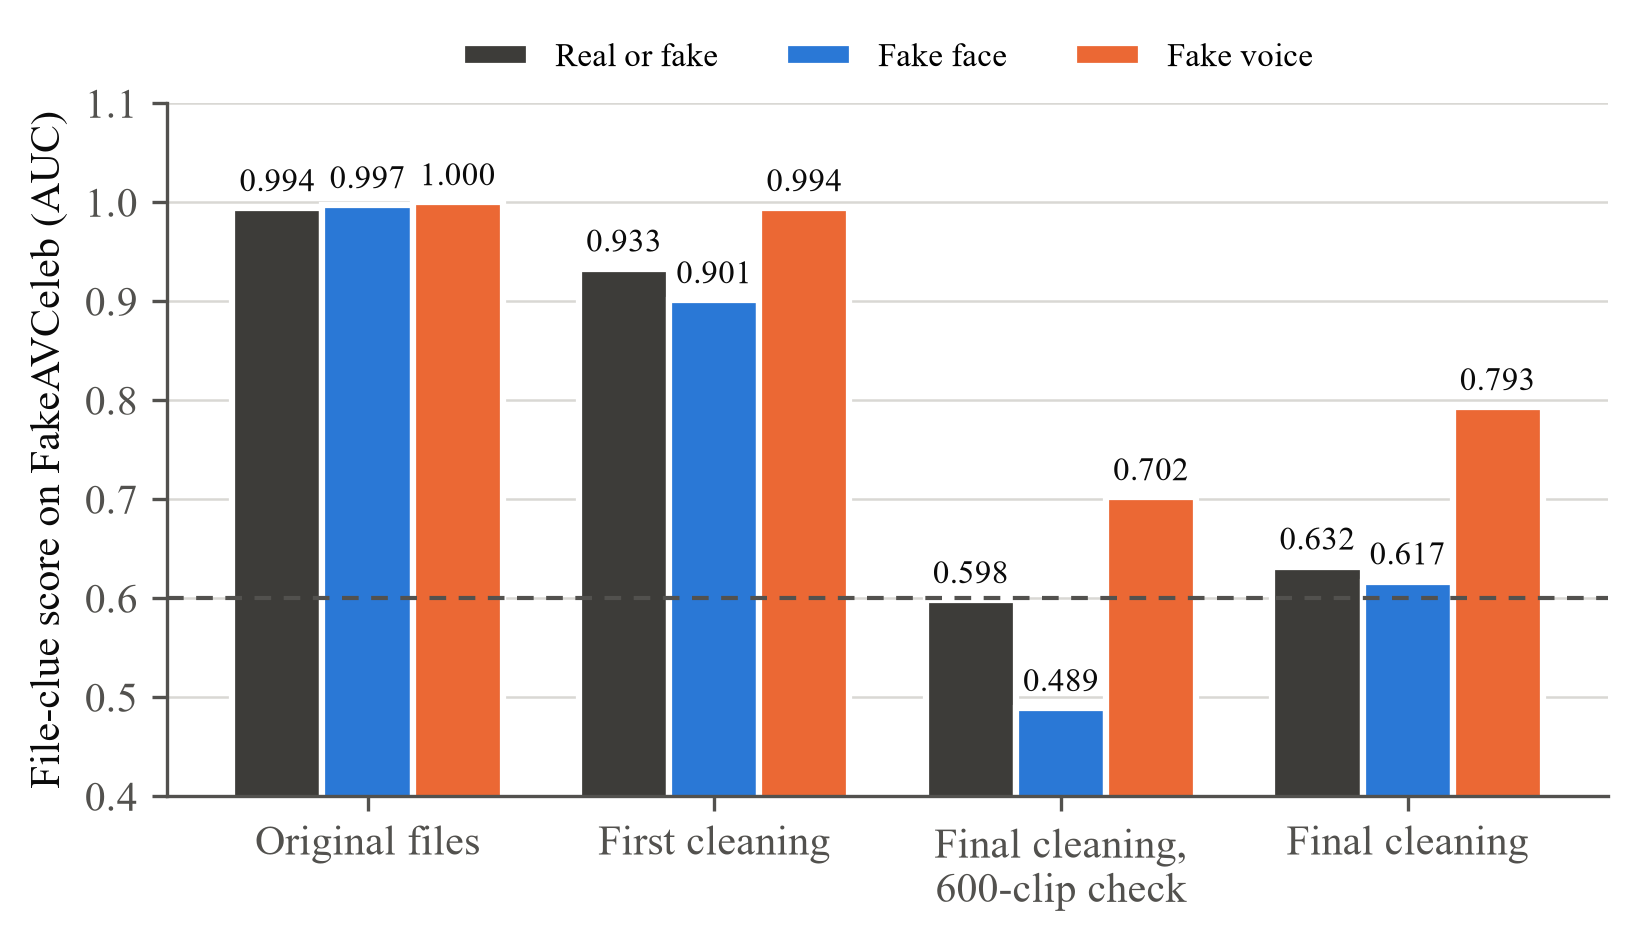
\includegraphics[width=0.85\textwidth,keepaspectratio]{fig_h1.png}
    \caption{Shortcut ceiling on FakeAVCeleb across neutralizer attempts, for the clip, video and audio labels. The dashed line is the preregistered bar.}
    \label{fig:h1}
\end{figure}

\textbf{H1 is not met.} On all of FakeAVCeleb, v4 gives a clip-label ceiling of
{{audit.fakeavceleb.neutral.clip}}, against a bar of 0.60. We report this as a
failed test, as P-001 requires. The check sample had passed. The full set did
not, and we did not tune the neutralizer again after seeing it.

The main residual cue is video bitrate. Every clip is encoded at the same
constant quality, so the encoder spends bits according to image content.
Smoother face-swapped faces compress into fewer bits. That makes bitrate a
property of the manipulated pixels, not of the generator's file pipeline. A
detector that reads the pixels may legitimately see the same smoothness. But
H1 was defined on all cues, so it fails as written.

The audio label keeps a higher ceiling, {{audit.fakeavceleb.neutral.audio}}.
It comes mainly from millisecond differences at the clip ends and from
loudness after AAC encoding. This residual matters for any claim about which
modality was faked, and P-001 requires us to report it beside H3.

\section{The Refusals Selection Effect}
\label{sec:refusals}

Neutralizer v4 refuses any clip with less than 3.00 s of sound. On FakeAVCeleb
it refused {{neutral.fakeavceleb.refused|int}} clips and kept
{{neutral.fakeavceleb.kept|int}}. Every refused clip carries generated speech.
No real clip was refused. Table~\ref{tab:census-fakeavceleb} shows where they
came from: the FakeVideo-FakeAudio category falls from
{{audit.fakeavceleb.raw.census.FakeVideo-FakeAudio.clips|int}} to
{{audit.fakeavceleb.neutral.census.FakeVideo-FakeAudio.clips|int}} clips, and
RealVideo-FakeAudio from
{{audit.fakeavceleb.raw.census.RealVideo-FakeAudio.clips|int}} to
{{audit.fakeavceleb.neutral.census.RealVideo-FakeAudio.clips|int}}.

This is a selection effect, and it has two consequences. First, the neutral
test set has fewer short generated-speech clips than the raw one, so neutral
and raw results describe different populations. Second, ``too short to
neutralize'' is itself a cue. A system that refused short clips would
implicitly flag generated speech. We do not use refusals as a signal. We
report the refusal count beside every result on these copies.

\section{How the Numbers Are Computed, and What Changed}

Numbers in this report are not directly comparable with numbers from the
project's earlier phases. Table~\ref{tab:changes} lists what changed in the
computation and why. None of these changes was chosen after seeing the result
it affects.

\begin{table}[ht]
    \centering
    \footnotesize
    \caption{Changes to how numbers are computed, from section 5.3 of the project handbook.}
    \label{tab:changes}
    \begin{tabularx}{\textwidth}{@{}>{\raggedright\arraybackslash}p{2.0cm} >{\raggedright\arraybackslash}p{2.2cm} >{\raggedright\arraybackslash}X >{\raggedright\arraybackslash}p{3.0cm} >{\raggedright\arraybackslash}p{3.2cm}@{}}
        \toprule
        \textbf{What} & \textbf{Before} & \textbf{Now} & \textbf{Why} & \textbf{Effect on comparison} \\
        \midrule
        EER & Nearest ROC point to FPR = FNR & Linear interpolation where FPR = FNR & The nearest point can be several points off on small sets & Old EERs can differ, most on small sets \\
        Decision threshold & Fixed 0.5 & Maximum balanced accuracy on validation; clip ids recorded; overlap refused & 0.5 means nothing on fake-heavy data & Old FPR, FNR and balanced accuracy are not comparable \\
        FF++ split & Grouped by source identity & Grouped by connected identity component & Donor faces crossed train and test & Old FF++ in-domain numbers were optimistic \\
        Identity-strict subset & A file name read as a person & File names are not identities & The old strict test had no RVFA clips & Old strict numbers covered three of four categories \\
        Input data & Raw files & Neutralizer v4 & Raw files leak the label ({{audit.fakeavceleb.raw.clip}}) & Neutral and raw numbers measure different things; {{neutral.fakeavceleb.refused|int}} short generated-speech clips refused \\
        Sync clip score & Not used & Mean window misfit $s$, reported as $1 - e^{-s}$ & Puts the score in $[0, 1)$ & Monotone, so AUC is unchanged; not a calibrated probability \\
        Shortcut ceiling & Did not exist & Gradient-boosted trees on file and audio-edge cues, five folds grouped by identity & The bar any detector must beat & Single-cue AUCs are slightly optimistic; the ceiling is out-of-fold \\
        False-alarm threshold (H4) & Did not exist & Split conformal rank $\lceil (n+1)(1-\alpha) \rceil$; Neyman-Pearson umbrella for $(\alpha, \delta)$ & Source thresholds break under shift & Standard published methods~\cite{bates2023,tong2018}, not new maths \\
        \bottomrule
    \end{tabularx}
\end{table}

Some things did not change. ROC-AUC is computed the same way. Intervals are
95\%, from 1,000 bootstrap resamples of identities, not clips~\cite{bootstrap}.
Clips of one person are not independent, so resampling clips would give
intervals that are too narrow. Every trained model uses three seeds, 17, 29
and 43.

%
\chapter{The Real-Only Sync Path}
\label{ch:sync}

\section{Why a Real-Only Sync Path}

A lip-sync detector asks one question: do the lips match the sound? Many
audio-visual fakes break that match. A cloned voice laid over a real face says
words the lips never formed. A generated mouth driven by audio rarely tracks it
perfectly.

We train the sync path on real clips only, for one reason. A model that never
sees a fake cannot learn what a particular generator's files look like. It can
only learn what real speech looks like, and flag clips that depart from it. On
data that still carries a residual shortcut, that is the safest design we
know. AVH-Align~\cite{smeu2025} showed the same idea holds up when the silence
shortcut is removed.

\section{Pipeline}

Figure~\ref{fig:pipeline} shows the full method.

\begin{figure}[htbp]
    \centering
    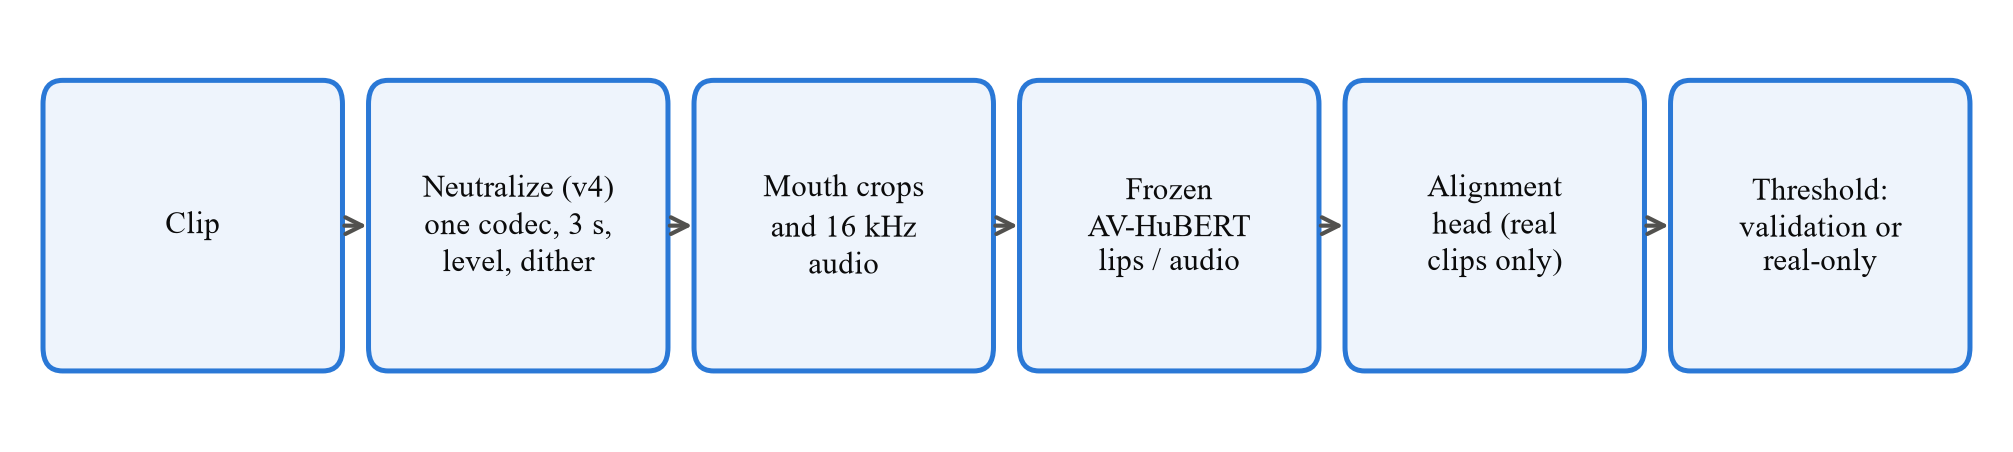
\includegraphics[width=0.95\textwidth,keepaspectratio]{fig_pipeline.png}
    \caption{Method overview. Each clip is neutralized, cut into mouth crops and audio, encoded by frozen AV-HuBERT, scored by an alignment head trained on real clips only, and thresholded either on source validation or on real target clips.}
    \label{fig:pipeline}
\end{figure}

\begin{enumerate}
    \item \textbf{Neutral clip.} Each clip comes from neutralizer v4: 3.00 s,
    25 fps video, 16 kHz audio.
    \item \textbf{Mouth crops.} MediaPipe's Face Landmarker finds facial
    landmarks in every frame. A similarity transform levels the eye line,
    scales the distance between the eyes to a fixed value, and puts the mouth
    centre in the middle of the crop. Angle, scale and centre are smoothed over
    neighbouring frames so the crop does not jitter. The result is an 88 by 88
    grey crop per frame, the input AV-HuBERT expects.
    \item \textbf{Windows.} Each clip gives two 2-second windows, starting at
    0 s and 1 s. A window needs a face in at least 80\% of its frames.
    \item \textbf{Frozen AV-HuBERT.} AV-HuBERT Base~\cite{avhubert} encodes
    each window twice: once with lips only (audio zeroed) and once with audio
    only. Each pass gives 50 frames of 768-dimensional features. The encoder
    is never trained.
    \item \textbf{Alignment head.} A small network scores each pair of lip and
    audio frames at the same instant.
    \item \textbf{Clip score.} The mean misfit over frames and windows.
\end{enumerate}

\section{The Alignment Head}

For a lips feature $l$ and an audio feature $a$ at the same frame, the head
builds the vector $[l, a, l \odot a, |l - a|]$. It applies layer
normalization, a linear layer to 256 units, a GELU and a final linear layer to
one logit $g$. A high logit means the two frames belong together.

\subsection{Training loss}

The head trains on real clips only, with a binary cross-entropy loss. Each
batch has three kinds of pair:

\begin{itemize}
    \item \textbf{Aligned:} lips and audio from the same instant of the same
    real clip. Target 1.
    \item \textbf{Shifted:} the same lips with the audio rolled by a random 5
    to 20 frames, which is 200 to 800 ms. Target 0.
    \item \textbf{Foreign:} the same lips with audio from another clip in the
    batch. Target 0.
\end{itemize}

The loss is the mean of the positive and negative terms, weighted equally.
Shifted pairs teach the head about timing. Foreign pairs teach it about
content: the right sounds for the mouth shapes. Training uses AdamW with a
learning rate of $10^{-3}$ and weight decay of $10^{-4}$ for 10 epochs, at
seeds 17, 29 and 43.

\subsection{Epoch selection}

We keep the epoch with the lowest alignment loss on real validation clips. No
fake label is read during training or selection. Fake labels are read only
when the frozen head scores the validation and test sets. This rule matters.
In the project's earlier phases, selection on the wrong quantity kept a
below-chance checkpoint (Chapter~\ref{ch:history}).

\subsection{Clip score}

A window's score is its mean misfit over aligned frames,
\[
    s_{\mathrm{window}} = \frac{1}{T} \sum_{t=1}^{T} -\log \sigma(g_t),
\]
where $\sigma$ is the logistic function and $T = 50$. A clip's score $s$ is the
mean over its windows. For the evaluation tools we report $1 - e^{-s}$, which
lies in $[0, 1)$ and keeps the order of the scores. AUC is therefore unchanged.
The score is not a calibrated probability.

\section{In-Domain Results}

Table~\ref{tab:sync-indomain} gives the results on neutral FakeAVCeleb. Every
clip in every set had a usable window, so coverage is complete.

\begin{table}[ht]
    \centering
    \small
    \caption{Sync path on neutral FakeAVCeleb. ROC-AUC with 95\% identity-bootstrap intervals; balanced accuracy and FPR at the threshold chosen on validation.}
    \label{tab:sync-indomain}
    \begin{tabular}{l l r l r r}
        \toprule
        \textbf{Set} & \textbf{Seed} & \textbf{Clips} & \textbf{AUC [95\% CI]} & \textbf{Bal. acc.} & \textbf{FPR} \\
        \midrule
        Validation & 17 & {{sync.val.seed17.n|int}} & {{sync.val.seed17.auc}} [{{sync.val.seed17.auc_low}}, {{sync.val.seed17.auc_high}}] & {{sync.val.seed17.balanced_accuracy}} & {{sync.val.seed17.fpr}} \\
                   & 29 & {{sync.val.seed29.n|int}} & {{sync.val.seed29.auc}} [{{sync.val.seed29.auc_low}}, {{sync.val.seed29.auc_high}}] & {{sync.val.seed29.balanced_accuracy}} & {{sync.val.seed29.fpr}} \\
                   & 43 & {{sync.val.seed43.n|int}} & {{sync.val.seed43.auc}} [{{sync.val.seed43.auc_low}}, {{sync.val.seed43.auc_high}}] & {{sync.val.seed43.balanced_accuracy}} & {{sync.val.seed43.fpr}} \\
        \midrule
        Test & 17 & {{sync.test.seed17.n|int}} & {{sync.test.seed17.auc}} [{{sync.test.seed17.auc_low}}, {{sync.test.seed17.auc_high}}] & {{sync.test.seed17.balanced_accuracy}} & {{sync.test.seed17.fpr}} \\
             & 29 & {{sync.test.seed29.n|int}} & {{sync.test.seed29.auc}} [{{sync.test.seed29.auc_low}}, {{sync.test.seed29.auc_high}}] & {{sync.test.seed29.balanced_accuracy}} & {{sync.test.seed29.fpr}} \\
             & 43 & {{sync.test.seed43.n|int}} & {{sync.test.seed43.auc}} [{{sync.test.seed43.auc_low}}, {{sync.test.seed43.auc_high}}] & {{sync.test.seed43.balanced_accuracy}} & {{sync.test.seed43.fpr}} \\
        \midrule
        Identity-strict & 17 & {{sync.test-identity-strict.seed17.n|int}} & {{sync.test-identity-strict.seed17.auc}} [{{sync.test-identity-strict.seed17.auc_low}}, {{sync.test-identity-strict.seed17.auc_high}}] & {{sync.test-identity-strict.seed17.balanced_accuracy}} & {{sync.test-identity-strict.seed17.fpr}} \\
        test            & 29 & {{sync.test-identity-strict.seed29.n|int}} & {{sync.test-identity-strict.seed29.auc}} [{{sync.test-identity-strict.seed29.auc_low}}, {{sync.test-identity-strict.seed29.auc_high}}] & {{sync.test-identity-strict.seed29.balanced_accuracy}} & {{sync.test-identity-strict.seed29.fpr}} \\
                        & 43 & {{sync.test-identity-strict.seed43.n|int}} & {{sync.test-identity-strict.seed43.auc}} [{{sync.test-identity-strict.seed43.auc_low}}, {{sync.test-identity-strict.seed43.auc_high}}] & {{sync.test-identity-strict.seed43.balanced_accuracy}} & {{sync.test-identity-strict.seed43.fpr}} \\
        \bottomrule
    \end{tabular}
\end{table}

Three readings follow from the table.

\textbf{The result holds across seeds.} Test AUC is
{{sync.test.seed17.auc}}, {{sync.test.seed29.auc}} and
{{sync.test.seed43.auc}}. The three intervals overlap. In earlier phases of
this project, the seed alone moved results more than the effects being
claimed. So we read the three seeds together and do not pick one.

\textbf{The result holds on the identity-strict subset.} On test clips whose
every named person is in the test partition only, AUC is
{{sync.test-identity-strict.seed17.auc}},
{{sync.test-identity-strict.seed29.auc}} and
{{sync.test-identity-strict.seed43.auc}}. The sync path is not scoring well by
recognizing people it trained on.

\textbf{The result sits above the shortcut ceiling of the same copies.} The
ceiling on neutral FakeAVCeleb is {{audit.fakeavceleb.neutral.clip}}. All
three seeds score above it on the test set. File cues alone cannot explain
the sync path's result. This comparison matters more than the raw AUC: a
detector on raw FakeAVCeleb would have to beat {{audit.fakeavceleb.raw.clip}}
to show the same thing.

\section{Results by Manipulation Method}

The strongest evidence that the sync path reads lip and audio agreement comes
from its pattern across methods. Table~\ref{tab:sync-methods} gives test AUC
per method, where each method's fakes are ranked against all real test clips.
Figure~\ref{fig:sync-methods} plots the same numbers.

\begin{table}[ht]
    \centering
    \small
    \caption{Sync path test AUC per manipulation method, neutral FakeAVCeleb, against all real test clips.}
    \label{tab:sync-methods}
    \begin{tabular}{l l r r r}
        \toprule
        \textbf{Method} & \textbf{What changes} & \textbf{Seed 17} & \textbf{Seed 29} & \textbf{Seed 43} \\
        \midrule
        RTVC                & Voice cloned; real face & {{sync.test.seed17.method.rtvc}} & {{sync.test.seed29.method.rtvc}} & {{sync.test.seed43.method.rtvc}} \\
        FaceSwap + Wav2Lip  & Face and mouth regenerated & {{sync.test.seed17.method.faceswap-wav2lip}} & {{sync.test.seed29.method.faceswap-wav2lip}} & {{sync.test.seed43.method.faceswap-wav2lip}} \\
        FSGAN + Wav2Lip     & Face and mouth regenerated & {{sync.test.seed17.method.fsgan-wav2lip}} & {{sync.test.seed29.method.fsgan-wav2lip}} & {{sync.test.seed43.method.fsgan-wav2lip}} \\
        Wav2Lip             & Mouth regenerated & {{sync.test.seed17.method.wav2lip}} & {{sync.test.seed29.method.wav2lip}} & {{sync.test.seed43.method.wav2lip}} \\
        FSGAN               & Face swapped; lips and voice kept & {{sync.test.seed17.method.fsgan}} & {{sync.test.seed29.method.fsgan}} & {{sync.test.seed43.method.fsgan}} \\
        FaceSwap            & Face swapped; lips and voice kept & {{sync.test.seed17.method.faceswap}} & {{sync.test.seed29.method.faceswap}} & {{sync.test.seed43.method.faceswap}} \\
        \bottomrule
    \end{tabular}
\end{table}

\begin{figure}[htbp]
    \centering
    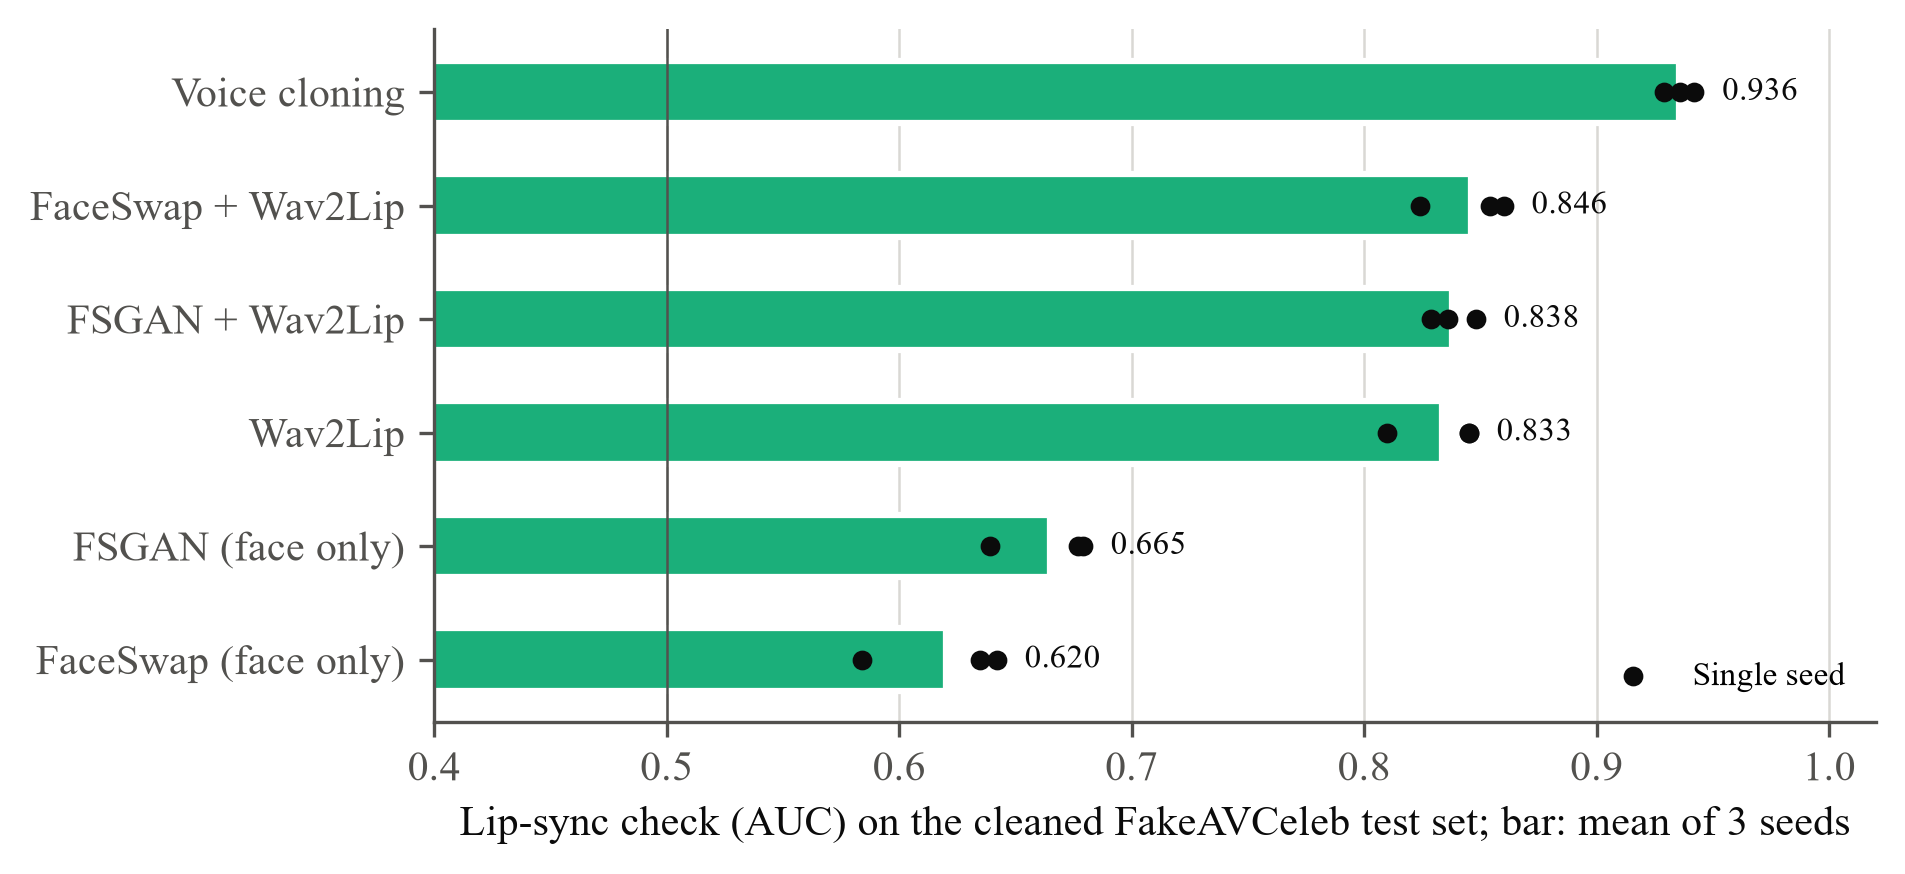
\includegraphics[width=0.85\textwidth,keepaspectratio]{fig_sync_methods.png}
    \caption{Sync path AUC per manipulation method on neutral FakeAVCeleb test, three seeds.}
    \label{fig:sync-methods}
\end{figure}

The order is the one the mechanism predicts.

\begin{itemize}
    \item \textbf{Voice cloning is caught best.} RTVC puts a new voice over the
    original face. The lips still move for the original words, so the
    mismatch between lips and sound is large.
    \item \textbf{Wav2Lip comes next.} Wav2Lip regenerates the mouth to follow
    the audio. Its fit is close but imperfect, so some misfit remains.
    \item \textbf{Face swap alone is caught least.} FaceSwap and FSGAN replace
    the face but keep the original mouth motion and the original voice. The
    lips and the sound still agree, so a sync model has little to find.
\end{itemize}

A model that had learned a shortcut would not need to follow this order. A
codec or silence cue attaches to a file pipeline, not to how much the lips and
sound disagree. The sync path never saw a fake and never saw a label during
training, so it had no way to learn which pipeline made which fake. Its errors
fall where its design says they should: on fakes that leave the lip-sound
match intact. This order is evidence that the path reads lip and audio
agreement, not proof; the caveat below gives the main alternative. A complete
detector needs a second path for face swaps. That is the visual path, which
Chapter~\ref{ch:h2} tests.

The same order holds on the identity-strict subset
(Table~\ref{tab:sync-methods-strict}).

\begin{table}[ht]
    \centering
    \small
    \caption{Sync path AUC per manipulation method, identity-strict test subset.}
    \label{tab:sync-methods-strict}
    \begin{tabular}{l r r r}
        \toprule
        \textbf{Method} & \textbf{Seed 17} & \textbf{Seed 29} & \textbf{Seed 43} \\
        \midrule
        RTVC               & {{sync.test-identity-strict.seed17.method.rtvc}} & {{sync.test-identity-strict.seed29.method.rtvc}} & {{sync.test-identity-strict.seed43.method.rtvc}} \\
        FaceSwap + Wav2Lip & {{sync.test-identity-strict.seed17.method.faceswap-wav2lip}} & {{sync.test-identity-strict.seed29.method.faceswap-wav2lip}} & {{sync.test-identity-strict.seed43.method.faceswap-wav2lip}} \\
        FSGAN + Wav2Lip    & {{sync.test-identity-strict.seed17.method.fsgan-wav2lip}} & {{sync.test-identity-strict.seed29.method.fsgan-wav2lip}} & {{sync.test-identity-strict.seed43.method.fsgan-wav2lip}} \\
        Wav2Lip            & {{sync.test-identity-strict.seed17.method.wav2lip}} & {{sync.test-identity-strict.seed29.method.wav2lip}} & {{sync.test-identity-strict.seed43.method.wav2lip}} \\
        FSGAN              & {{sync.test-identity-strict.seed17.method.fsgan}} & {{sync.test-identity-strict.seed29.method.fsgan}} & {{sync.test-identity-strict.seed43.method.fsgan}} \\
        FaceSwap           & {{sync.test-identity-strict.seed17.method.faceswap}} & {{sync.test-identity-strict.seed29.method.faceswap}} & {{sync.test-identity-strict.seed43.method.faceswap}} \\
        \bottomrule
    \end{tabular}
\end{table}

One caveat applies. The audio label on the neutral copies keeps a residual
ceiling of {{audit.fakeavceleb.neutral.audio}}. The sync path reads audio, so
in principle part of its misfit on cloned voices could come from audio
properties rather than from the lips. Real-only training makes this less
likely, because nothing in training rewards it. It does not rule it out.
Amendment A16 tested the mechanism directly: moving the audio of real clips
raises the misfit, even by one frame (Section~\ref{sec:overnight}). It did not
test cloned voices, which are new audio rather than moved audio.

\section{The Weak Point: False Alarms}

The sync path ranks clips well, but its threshold flags many real clips. At
the threshold chosen on validation, the false-positive rate on real test clips
is {{sync.test.seed17.fpr}}, {{sync.test.seed29.fpr}} and
{{sync.test.seed43.fpr}} for the three seeds. On validation the same
thresholds give {{sync.val.seed17.fpr}}, {{sync.val.seed29.fpr}} and
{{sync.val.seed43.fpr}}.

Two things drive this. The threshold maximizes balanced accuracy, which trades
false alarms against missed fakes equally. And FakeAVCeleb has few real clips,
so the real side of the validation set is small and the threshold moves from
seed to seed. A deployed detector would face a worse version of the problem.
It would carry this threshold to new footage whose real clips score
differently. That is the question H4 asks, in the next chapter.

%
\chapter{Cross-Corpus Evaluation and False-Alarm Control}
\label{ch:crosscorpus}

This chapter tests the frozen sync path on data it never saw, and tests
whether a threshold set from real clips of a new domain holds its
false-positive rate.

\section{Setup}

Nothing is retrained for these tests. The three sync heads from
Chapter~\ref{ch:sync}, one per seed, are frozen. Each target corpus goes
through the same steps as FakeAVCeleb:

\begin{enumerate}
    \item neutralizer v4, with one frame size per corpus (1280x720 for
    HiFi-AVDF);
    \item MediaPipe mouth crops and frozen AV-HuBERT features, two 2-second
    windows per clip;
    \item scoring by each frozen head;
    \item evaluation at the source threshold chosen on FakeAVCeleb
    validation, with 1,000 bootstrap resamples for the interval;
    \item a shortcut audit of the neutral copies, so each result sits beside
    the ceiling of the same data.
\end{enumerate}

The targets are the LAV-DF test sample (1,000 original recordings with all
their edits, 3,823 files), the DFDC subset, and HiFi-AVDF. All three are
locked. They train, select and calibrate nothing, except that H4 draws real
calibration clips from the target by design.

LAV-DF needs two labels. The neutral copy keeps 3.00 s from the first sound,
but LAV-DF edits single words anywhere in a longer recording. In 1,307 of the
2,823 fake clips, the kept window contains no edited time at all, so under the
file label they are real footage labelled fake. We found this after reading
the file-label results for the sync path and H4. Amendment A9 adds a window
label: a clip is fake if its kept window overlaps edited time by at least one
frame. Every LAV-DF result below is reported under both labels. H2, which had
not run, uses the window label.

\section{Shortcut Ceilings of the Target Copies}

Table~\ref{tab:target-ceilings} gives the ceiling of each target on raw files
and on its neutral copy. A cross-corpus AUC should be read against the neutral
ceiling of the same corpus, not against 0.5.

\begin{table}[ht]
    \centering
    \small
    \caption{Shortcut ceilings of the cross-corpus targets, raw and neutral. DFDC has clip labels only.}
    \label{tab:target-ceilings}
    \begin{tabular}{l r r r r r r}
        \toprule
         & \multicolumn{3}{c}{\textbf{Raw}} & \multicolumn{3}{c}{\textbf{Neutral}} \\
        \textbf{Corpus} & \textbf{Clip} & \textbf{Video} & \textbf{Audio} & \textbf{Clip} & \textbf{Video} & \textbf{Audio} \\
        \midrule
        LAV-DF, file label & {{audit.lavdf.raw.clip}} & {{audit.lavdf.raw.video}} & {{audit.lavdf.raw.audio}} & {{audit.lavdf.neutral.clip}} & {{audit.lavdf.neutral.video}} & {{audit.lavdf.neutral.audio}} \\
        LAV-DF, window label & {{audit.lavdf.raw.clip}} & {{audit.lavdf.raw.video}} & {{audit.lavdf.raw.audio}} & {{audit.lavdf.window.clip}} & {{audit.lavdf.window.video}} & {{audit.lavdf.window.audio}} \\
        DFDC      & {{audit.dfdc.raw.clip}} & {{audit.dfdc.raw.video}} & n/a & {{audit.dfdc.neutral.clip}} & n/a & n/a \\
        HiFi-AVDF & {{audit.hifiavdf.raw.clip}} & {{audit.hifiavdf.raw.video}} & {{audit.hifiavdf.raw.audio}} & {{audit.hifiavdf.neutral.clip}} & {{audit.hifiavdf.neutral.video}} & {{audit.hifiavdf.neutral.audio}} \\
        \bottomrule
    \end{tabular}
\end{table}

The LAV-DF raw audit used a stratified sample of files, and the neutral audit
uses the test sample. The two populations overlap but are not identical.

\section{Sync Path Across Corpora}

Table~\ref{tab:cross-corpus} gives the frozen sync path's results on each
target, for each seed. Figure~\ref{fig:cross-corpus} plots the AUC per target,
with HiFi-AVDF also split by generator.

\begin{table}[ht]
    \centering
    \small
    \caption{Frozen sync path on the cross-corpus targets. ROC-AUC with 95\% bootstrap intervals; balanced accuracy and FPR at the source threshold.}
    \label{tab:cross-corpus}
    \begin{tabular}{l l r l r r}
        \toprule
        \textbf{Target} & \textbf{Seed} & \textbf{Clips} & \textbf{AUC [95\% CI]} & \textbf{Bal. acc.} & \textbf{FPR} \\
        \midrule
        LAV-DF, file label & 17 & {{sync.lavdf-test.seed17.scored|int}} & {{sync.lavdf-test.seed17.auc}} [{{sync.lavdf-test.seed17.auc_low}}, {{sync.lavdf-test.seed17.auc_high}}] & {{sync.lavdf-test.seed17.balanced_accuracy}} & {{sync.lavdf-test.seed17.fpr}} \\
                    & 29 & {{sync.lavdf-test.seed29.scored|int}} & {{sync.lavdf-test.seed29.auc}} [{{sync.lavdf-test.seed29.auc_low}}, {{sync.lavdf-test.seed29.auc_high}}] & {{sync.lavdf-test.seed29.balanced_accuracy}} & {{sync.lavdf-test.seed29.fpr}} \\
                    & 43 & {{sync.lavdf-test.seed43.scored|int}} & {{sync.lavdf-test.seed43.auc}} [{{sync.lavdf-test.seed43.auc_low}}, {{sync.lavdf-test.seed43.auc_high}}] & {{sync.lavdf-test.seed43.balanced_accuracy}} & {{sync.lavdf-test.seed43.fpr}} \\
        \midrule
        LAV-DF, window label & 17 & {{sync.lavdf-window.seed17.scored|int}} & {{sync.lavdf-window.seed17.auc}} [{{sync.lavdf-window.seed17.auc_low}}, {{sync.lavdf-window.seed17.auc_high}}] & {{sync.lavdf-window.seed17.balanced_accuracy}} & {{sync.lavdf-window.seed17.fpr}} \\
                    & 29 & {{sync.lavdf-window.seed29.scored|int}} & {{sync.lavdf-window.seed29.auc}} [{{sync.lavdf-window.seed29.auc_low}}, {{sync.lavdf-window.seed29.auc_high}}] & {{sync.lavdf-window.seed29.balanced_accuracy}} & {{sync.lavdf-window.seed29.fpr}} \\
                    & 43 & {{sync.lavdf-window.seed43.scored|int}} & {{sync.lavdf-window.seed43.auc}} [{{sync.lavdf-window.seed43.auc_low}}, {{sync.lavdf-window.seed43.auc_high}}] & {{sync.lavdf-window.seed43.balanced_accuracy}} & {{sync.lavdf-window.seed43.fpr}} \\
        \midrule
        DFDC & 17 & {{sync.dfdc.seed17.scored|int}} & {{sync.dfdc.seed17.auc}} [{{sync.dfdc.seed17.auc_low}}, {{sync.dfdc.seed17.auc_high}}] & {{sync.dfdc.seed17.balanced_accuracy}} & {{sync.dfdc.seed17.fpr}} \\
             & 29 & {{sync.dfdc.seed29.scored|int}} & {{sync.dfdc.seed29.auc}} [{{sync.dfdc.seed29.auc_low}}, {{sync.dfdc.seed29.auc_high}}] & {{sync.dfdc.seed29.balanced_accuracy}} & {{sync.dfdc.seed29.fpr}} \\
             & 43 & {{sync.dfdc.seed43.scored|int}} & {{sync.dfdc.seed43.auc}} [{{sync.dfdc.seed43.auc_low}}, {{sync.dfdc.seed43.auc_high}}] & {{sync.dfdc.seed43.balanced_accuracy}} & {{sync.dfdc.seed43.fpr}} \\
        \midrule
        HiFi-AVDF & 17 & {{sync.hifiavdf.seed17.scored|int}} & {{sync.hifiavdf.seed17.auc}} [{{sync.hifiavdf.seed17.auc_low}}, {{sync.hifiavdf.seed17.auc_high}}] & {{sync.hifiavdf.seed17.balanced_accuracy}} & {{sync.hifiavdf.seed17.fpr}} \\
                  & 29 & {{sync.hifiavdf.seed29.scored|int}} & {{sync.hifiavdf.seed29.auc}} [{{sync.hifiavdf.seed29.auc_low}}, {{sync.hifiavdf.seed29.auc_high}}] & {{sync.hifiavdf.seed29.balanced_accuracy}} & {{sync.hifiavdf.seed29.fpr}} \\
                  & 43 & {{sync.hifiavdf.seed43.scored|int}} & {{sync.hifiavdf.seed43.auc}} [{{sync.hifiavdf.seed43.auc_low}}, {{sync.hifiavdf.seed43.auc_high}}] & {{sync.hifiavdf.seed43.balanced_accuracy}} & {{sync.hifiavdf.seed43.fpr}} \\
        \bottomrule
    \end{tabular}
\end{table}

\begin{figure}[htbp]
    \centering
    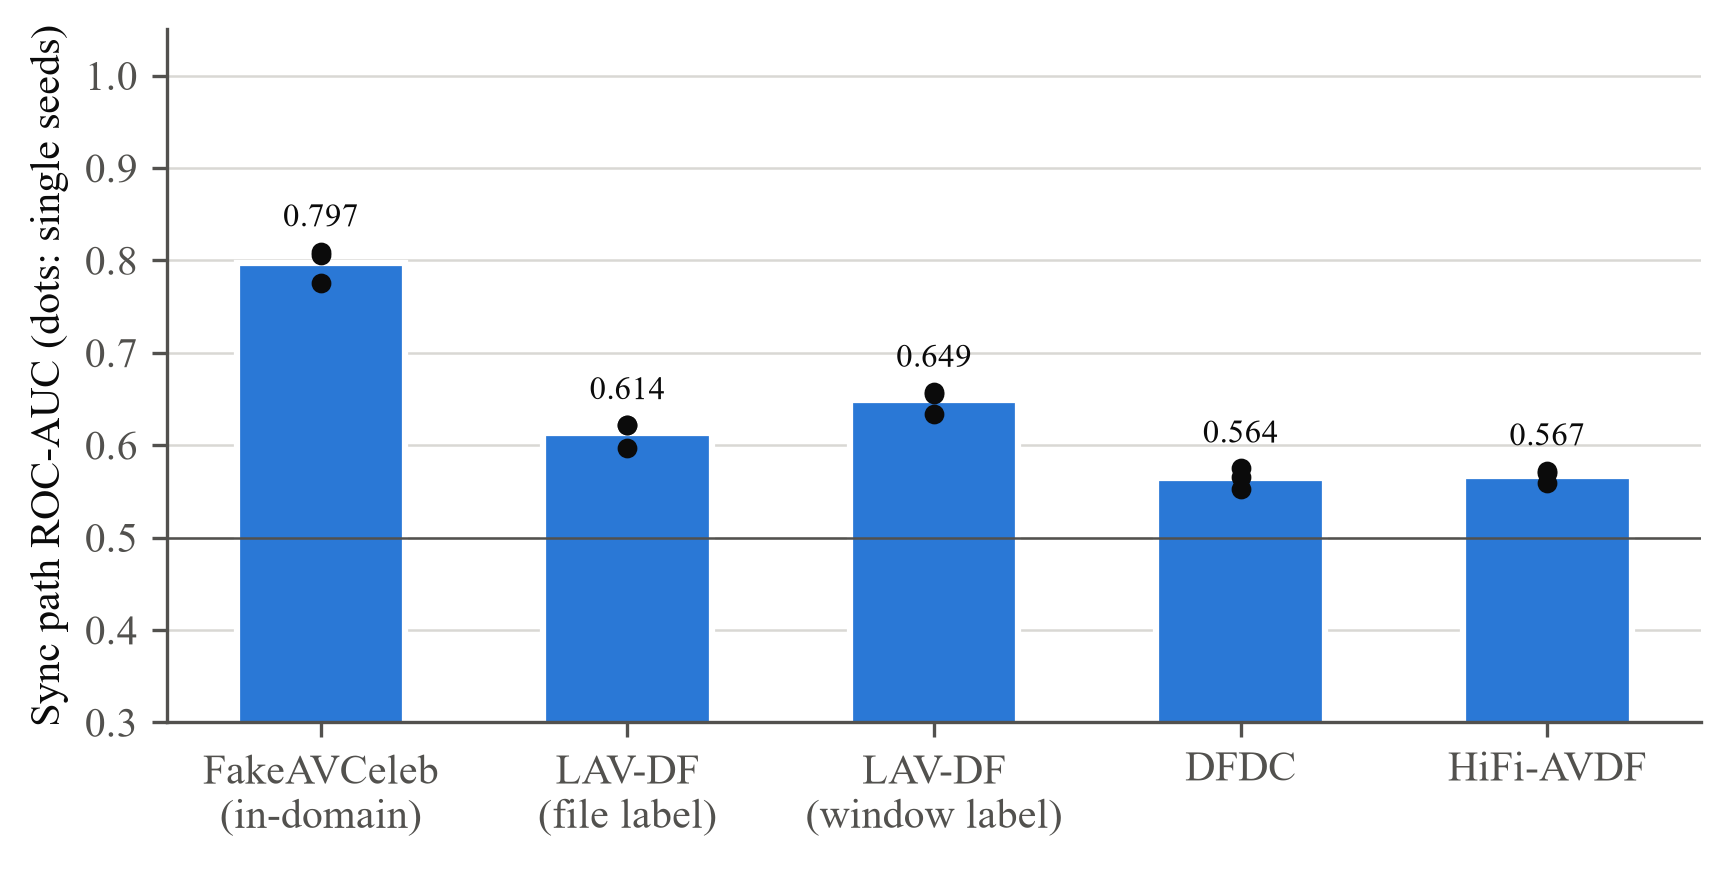
\includegraphics[width=0.9\textwidth,keepaspectratio]{fig_cross_corpus.png}
    \caption{Frozen sync path AUC per target corpus and per HiFi-AVDF generator, three seeds.}
    \label{fig:cross-corpus}
\end{figure}

Each target tests something different. LAV-DF edits only a few words inside a
real recording, so most of each 3-second clip may be untouched. DFDC's fakes
are mainly face swaps, the case the sync path catches least in-domain. HiFi-AVDF's generators make the whole clip, picture and sound
together. The FPR column shows how the source threshold behaves on each new
domain.

\subsection{HiFi-AVDF by generator}

Table~\ref{tab:hifi-generators} splits the HiFi-AVDF result by generator. Each
generator's clips are ranked against all real HiFi-AVDF clips.

\begin{table}[ht]
    \centering
    \small
    \caption{Frozen sync path AUC on HiFi-AVDF, per generator.}
    \label{tab:hifi-generators}
    \begin{tabular}{l r r r}
        \toprule
        \textbf{Generator} & \textbf{Seed 17} & \textbf{Seed 29} & \textbf{Seed 43} \\
        \midrule
        Kling 2.5    & {{sync.hifiavdf.seed17.method.kling2.5}} & {{sync.hifiavdf.seed29.method.kling2.5}} & {{sync.hifiavdf.seed43.method.kling2.5}} \\
        PixVerse V5  & {{sync.hifiavdf.seed17.method.pixverseV5}} & {{sync.hifiavdf.seed29.method.pixverseV5}} & {{sync.hifiavdf.seed43.method.pixverseV5}} \\
        Seedance 1.0 & {{sync.hifiavdf.seed17.method.seedance1.0}} & {{sync.hifiavdf.seed29.method.seedance1.0}} & {{sync.hifiavdf.seed43.method.seedance1.0}} \\
        Sora 2       & {{sync.hifiavdf.seed17.method.sora2}} & {{sync.hifiavdf.seed29.method.sora2}} & {{sync.hifiavdf.seed43.method.sora2}} \\
        Veo 3.1      & {{sync.hifiavdf.seed17.method.veo3.1}} & {{sync.hifiavdf.seed29.method.veo3.1}} & {{sync.hifiavdf.seed43.method.veo3.1}} \\
        Wan 2.5      & {{sync.hifiavdf.seed17.method.wan2.5}} & {{sync.hifiavdf.seed29.method.wan2.5}} & {{sync.hifiavdf.seed43.method.wan2.5}} \\
        \bottomrule
    \end{tabular}
\end{table}

These generators were released long after FakeAVCeleb was made. The sync path
never saw any of them, nor any fake at all. Its result on each one measures
how well that generator matches lip motion to speech, as judged by a model of
real speech.

\subsection{What the results show}

The sync path keeps some signal on every target, but far less than on
FakeAVCeleb, where it was trained. On LAV-DF it clears the neutral ceiling
under both labels. On DFDC, where every fake keeps its original voice, it sits
just above the ceiling of {{audit.dfdc.neutral.clip}}, and the seed-17
interval includes it. On HiFi-AVDF it falls
below the neutral ceiling of {{audit.hifiavdf.neutral.clip}}, so the bitrate
left after cleaning says more about the label than the lips do.

The generators explain why. PixVerse V5 is caught best
({{sync.hifiavdf.seed17.method.pixverseV5}} at seed 17). Veo 3.1 sits near
chance ({{sync.hifiavdf.seed17.method.veo3.1}}), and Sora 2 falls below it
({{sync.hifiavdf.seed17.method.sora2}}). These tools make sound and picture
together, so lips and voice already match. On Sora 2 the generated clips look
more in sync than the real ones. A detector built on lip-voice mismatch has
nothing to find there. That is a limit of the idea, not only of our model.

\subsection{Coverage, before and after amendment A10}

The face landmarker first found a face in only 2,110 of 6,064 DFDC windows,
because DFDC faces are small in full-HD frames. The sync path then scored 921
DFDC clips, 67 of them real. Amendment A10 locates the face with a second
detector first, only for windows that fall below the face bar. DFDC coverage
rose to {{sync.dfdc.seed17.scored|int}} clips, and HiFi-AVDF to
{{sync.hifiavdf.seed17.scored|int}}. AUC changed little; the intervals
narrowed. The tables show the results after A10. Both versions are in
\texttt{results/}.

Two smaller gaps remain. HiFi-AVDF has
{{audit.hifiavdf.raw.census.RealVideo-RealAudio.audio_codec.none|int}} real and
{{audit.hifiavdf.raw.census.FakeVideo-FakeAudio.audio_codec.none|int}} generated
source clips with no audio track, which a sync path cannot score. A few
neutral clips also have less video than audio, so some of their windows hold
fewer than 50 frames. Those windows are left out and counted, as windows
without a face already were.

\section{H4: False-Alarm Control From Real Clips}

\subsection{The question}

A deployed detector is usually tuned once, on the data it was built with, and
then run on new footage. If the new footage's real clips score differently,
the false-alarm rate changes and nobody notices. H4 asks whether a threshold
set from real clips of the new domain holds the false-positive rate where the
carried-over threshold does not.

\subsection{Three threshold rules}

For each target and seed, \texttt{scripts/run\_h4.py} compares three rules.

\begin{enumerate}
    \item \textbf{Source threshold.} The threshold chosen on FakeAVCeleb
    validation, applied unchanged. This is what a deployed detector would do.
    \item \textbf{Real-only conformal threshold.} A random set of
    $n_{\mathrm{cal}} = 200$ real target clips is set aside, using a seed
    fixed in P-001. The threshold is the score at rank
    $\lceil (n_{\mathrm{cal}}+1)(1-\alpha) \rceil$ among them, with
    $\alpha = 0.05$. For a new real clip from the same distribution, the
    chance of being flagged is then at most $\alpha$ on
    average~\cite{bates2023}.
    \item \textbf{Real-only umbrella threshold.} The Neyman-Pearson umbrella
    rule~\cite{tong2018} picks the lowest of the same real scores that is safe
    to use. Safe means its false-positive rate exceeds $\alpha$ with
    probability at most $\delta$. We use $\alpha = \delta = 0.05$. This is a stronger guarantee: it
    holds for this calibration draw with high probability, not only on
    average. It needs at least $\lceil \log\delta / \log(1-\alpha) \rceil = 59$
    real clips.
\end{enumerate}

No fake label is read to set any of these thresholds. All three are then
scored on the target clips that were not used for calibration. The
preregistered success rule is a realized FPR of at most $\alpha + 0.02 = 0.07$
with the conformal threshold, on every target.

\subsection{Targets}

H4 runs on LAV-DF test and HiFi-AVDF. It does not run on DFDC. Our DFDC subset
has only {{audit.dfdc.raw.census.RealVideo-RealAudio.clips|int}} real clips,
fewer than the 200 needed for calibration plus any held-out real clips to
score.

\subsection{Results}

Table~\ref{tab:h4} gives the realized false-positive and true-positive rates
of each rule, and Figure~\ref{fig:h4} plots the false-positive rates.

\begin{table}[ht]
    \centering
    \footnotesize
    \caption{H4: realized FPR and TPR on held-out target clips for each threshold rule. Success means conformal FPR at most 0.07.}
    \label{tab:h4}
    \begin{tabular}{l l r r r r r r l}
        \toprule
         & & \multicolumn{2}{c}{\textbf{Source}} & \multicolumn{2}{c}{\textbf{Conformal}} & \multicolumn{2}{c}{\textbf{Umbrella}} & \\
        \textbf{Target} & \textbf{Seed} & \textbf{FPR} & \textbf{TPR} & \textbf{FPR} & \textbf{TPR} & \textbf{FPR} & \textbf{TPR} & \textbf{Success} \\
        \midrule
        LAV-DF, file label & 17 & {{h4.lavdf-test-seed17.source_validation.fpr}} & {{h4.lavdf-test-seed17.source_validation.tpr}} & {{h4.lavdf-test-seed17.conformal_real_only.fpr}} & {{h4.lavdf-test-seed17.conformal_real_only.tpr}} & {{h4.lavdf-test-seed17.umbrella_real_only.fpr}} & {{h4.lavdf-test-seed17.umbrella_real_only.tpr}} & {{h4.lavdf-test-seed17.success}} \\
                    & 29 & {{h4.lavdf-test-seed29.source_validation.fpr}} & {{h4.lavdf-test-seed29.source_validation.tpr}} & {{h4.lavdf-test-seed29.conformal_real_only.fpr}} & {{h4.lavdf-test-seed29.conformal_real_only.tpr}} & {{h4.lavdf-test-seed29.umbrella_real_only.fpr}} & {{h4.lavdf-test-seed29.umbrella_real_only.tpr}} & {{h4.lavdf-test-seed29.success}} \\
                    & 43 & {{h4.lavdf-test-seed43.source_validation.fpr}} & {{h4.lavdf-test-seed43.source_validation.tpr}} & {{h4.lavdf-test-seed43.conformal_real_only.fpr}} & {{h4.lavdf-test-seed43.conformal_real_only.tpr}} & {{h4.lavdf-test-seed43.umbrella_real_only.fpr}} & {{h4.lavdf-test-seed43.umbrella_real_only.tpr}} & {{h4.lavdf-test-seed43.success}} \\
        \midrule
        LAV-DF, window label & 17 & {{h4.lavdf-window-seed17.source_validation.fpr}} & {{h4.lavdf-window-seed17.source_validation.tpr}} & {{h4.lavdf-window-seed17.conformal_real_only.fpr}} & {{h4.lavdf-window-seed17.conformal_real_only.tpr}} & {{h4.lavdf-window-seed17.umbrella_real_only.fpr}} & {{h4.lavdf-window-seed17.umbrella_real_only.tpr}} & {{h4.lavdf-window-seed17.success}} \\
                    & 29 & {{h4.lavdf-window-seed29.source_validation.fpr}} & {{h4.lavdf-window-seed29.source_validation.tpr}} & {{h4.lavdf-window-seed29.conformal_real_only.fpr}} & {{h4.lavdf-window-seed29.conformal_real_only.tpr}} & {{h4.lavdf-window-seed29.umbrella_real_only.fpr}} & {{h4.lavdf-window-seed29.umbrella_real_only.tpr}} & {{h4.lavdf-window-seed29.success}} \\
                    & 43 & {{h4.lavdf-window-seed43.source_validation.fpr}} & {{h4.lavdf-window-seed43.source_validation.tpr}} & {{h4.lavdf-window-seed43.conformal_real_only.fpr}} & {{h4.lavdf-window-seed43.conformal_real_only.tpr}} & {{h4.lavdf-window-seed43.umbrella_real_only.fpr}} & {{h4.lavdf-window-seed43.umbrella_real_only.tpr}} & {{h4.lavdf-window-seed43.success}} \\
        \midrule
        HiFi-AVDF & 17 & {{h4.hifiavdf-seed17.source_validation.fpr}} & {{h4.hifiavdf-seed17.source_validation.tpr}} & {{h4.hifiavdf-seed17.conformal_real_only.fpr}} & {{h4.hifiavdf-seed17.conformal_real_only.tpr}} & {{h4.hifiavdf-seed17.umbrella_real_only.fpr}} & {{h4.hifiavdf-seed17.umbrella_real_only.tpr}} & {{h4.hifiavdf-seed17.success}} \\
                  & 29 & {{h4.hifiavdf-seed29.source_validation.fpr}} & {{h4.hifiavdf-seed29.source_validation.tpr}} & {{h4.hifiavdf-seed29.conformal_real_only.fpr}} & {{h4.hifiavdf-seed29.conformal_real_only.tpr}} & {{h4.hifiavdf-seed29.umbrella_real_only.fpr}} & {{h4.hifiavdf-seed29.umbrella_real_only.tpr}} & {{h4.hifiavdf-seed29.success}} \\
                  & 43 & {{h4.hifiavdf-seed43.source_validation.fpr}} & {{h4.hifiavdf-seed43.source_validation.tpr}} & {{h4.hifiavdf-seed43.conformal_real_only.fpr}} & {{h4.hifiavdf-seed43.conformal_real_only.tpr}} & {{h4.hifiavdf-seed43.umbrella_real_only.fpr}} & {{h4.hifiavdf-seed43.umbrella_real_only.tpr}} & {{h4.hifiavdf-seed43.success}} \\
        \bottomrule
    \end{tabular}
\end{table}

\begin{figure}[htbp]
    \centering
    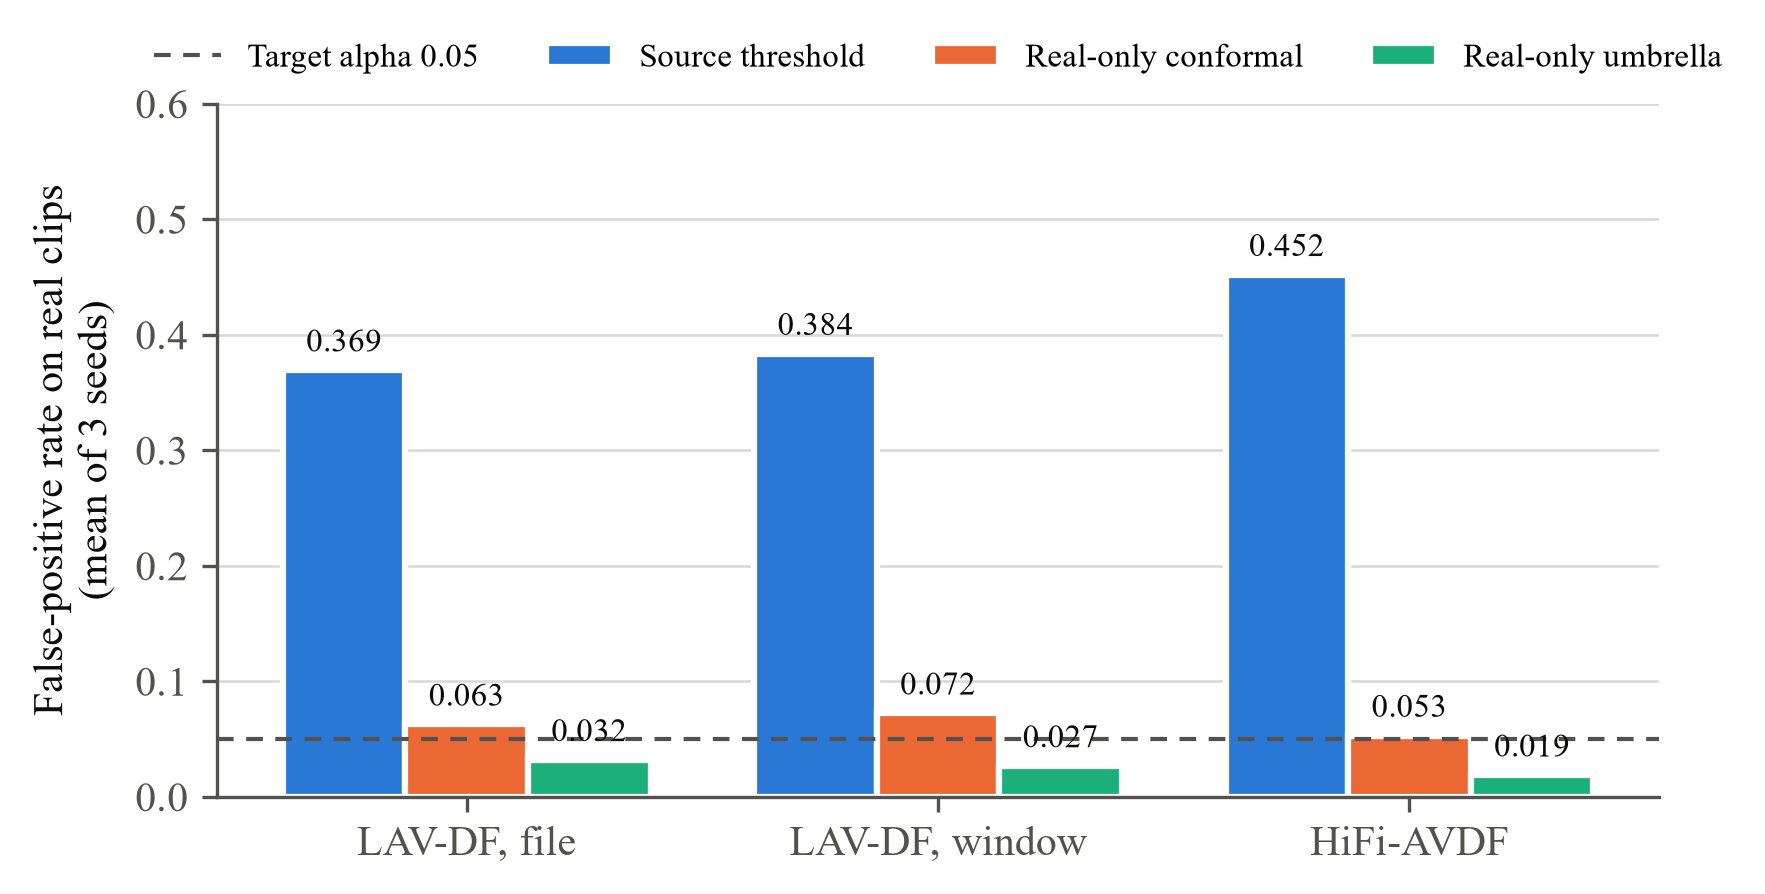
\includegraphics[width=0.85\textwidth,keepaspectratio]{fig_h4.png}
    \caption{Realized false-positive rate per threshold rule, target and seed. The dashed lines mark $\alpha = 0.05$ and the preregistered limit of 0.07.}
    \label{fig:h4}
\end{figure}

\subsection{How to read the table}

The source columns show what happens when the FakeAVCeleb threshold is carried
to a new domain unchanged. The conformal and umbrella columns show the
realized false-positive rate when the threshold comes from real target clips
alone. The success column applies the preregistered rule to the conformal
threshold. The TPR columns give the price of each rule: a threshold that flags
fewer real clips will also catch fewer fakes. With $n_{\mathrm{cal}} = 200$ and these
settings, the umbrella rule picks a higher rank than the conformal rule, so it
is the more conservative of the two.

Three limits apply to any reading of this table. First, the guarantees assume that
the calibration clips and the scored clips come from the same distribution.
Within one corpus that is reasonable. Across shifts inside a corpus it may not
hold. Second, each row uses one random calibration draw. The marginal
conformal guarantee holds on average over draws, so one draw can land above
$\alpha$ by chance. Third, H4 is a bar check, not a $p$-value test, so it sits
outside the Holm correction, which amendment A8 limits to H2's three targets.

\subsection{What H4 shows}

The threshold carried over from FakeAVCeleb does not transfer. It flags a large
share of real clips on every target. Set from 200 real target clips, the
conformal threshold brings the false-positive rate back near $\alpha$. H4 is
met on HiFi-AVDF in all three seeds, and on LAV-DF under the preregistered
file label in all three seeds.

Under the window label, which amendment A9 added after these results were
read, two of the three LAV-DF seeds land above the bar. The window label turns
clips cut from edited recordings into real clips. The calibration reals and
the scored reals may then no longer share one distribution, which is the
assumption the guarantee needs.

The price of control is recall. Near a 5\% false-positive rate, the sync path
catches {{h4.hifiavdf-seed17.conformal_real_only.tpr|pct}} of HiFi-AVDF fakes
and {{h4.lavdf-test-seed17.conformal_real_only.tpr|pct}} of LAV-DF fakes at
seed 17. Real-only calibration fixes the operating point. It cannot add signal
the detector does not have. A deployed system would need a stronger detector
under the same calibration. Chapter~\ref{ch:h2} tests whether fusing the
paths gives one.

%
\chapter{Fusion Against Visual-Only (H2)}
\label{ch:h2}

The first plan of this project fused three paths and expected the fusion to
beat any single path. The root study found no such gain across corpora, and
its fusion numbers turned out to be compromised (Chapter~\ref{ch:history}). This chapter runs
the comparison again, on neutral data, under rules fixed before any visual or
audio model existed.

\section{The Visual and Audio Paths}

The visual path is EfficientNet-B0~\cite{efficientnet} with a GRU over face
frames, trained on the video label. The audio path is Wav2Vec2
Base~\cite{wav2vec2} with attentive pooling, trained on the audio label. Both
train on the neutral FakeAVCeleb training partition, thinned to three
video-fake clips per real-video clip (amendment A1), at seeds 17, 29 and 43.
Each picks its epoch and its threshold on validation.

\begin{table}[htbp]
    \centering
    \caption{Visual and audio paths on the identity-strict neutral FakeAVCeleb
    test (ROC-AUC, 95\% identity-bootstrap interval), each on its own label}
    \label{tab:branches}
    \begin{tabular}{lll}
        \toprule
        \textbf{Seed} & \textbf{Visual (video label)} & \textbf{Audio (audio label)} \\
        \midrule
        17 & {{visual.test-identity-strict.seed17.auc}} [{{visual.test-identity-strict.seed17.auc_low}}, {{visual.test-identity-strict.seed17.auc_high}}] & {{audio.test-identity-strict.seed17.auc}} [{{audio.test-identity-strict.seed17.auc_low}}, {{audio.test-identity-strict.seed17.auc_high}}] \\
        29 & {{visual.test-identity-strict.seed29.auc}} [{{visual.test-identity-strict.seed29.auc_low}}, {{visual.test-identity-strict.seed29.auc_high}}] & {{audio.test-identity-strict.seed29.auc}} [{{audio.test-identity-strict.seed29.auc_low}}, {{audio.test-identity-strict.seed29.auc_high}}] \\
        43 & {{visual.test-identity-strict.seed43.auc}} [{{visual.test-identity-strict.seed43.auc_low}}, {{visual.test-identity-strict.seed43.auc_high}}] & {{audio.test-identity-strict.seed43.auc}} [{{audio.test-identity-strict.seed43.auc_low}}, {{audio.test-identity-strict.seed43.auc_high}}] \\
        \bottomrule
    \end{tabular}
\end{table}

\section{How the Fusion Is Fit}

Amendment A8 fixed every choice below on 16 November, before any visual or
audio checkpoint existed:

\begin{itemize}
    \item \textbf{Inputs.} Each path's logit for the clip. The sync logit is the
    logit of its probability. Each logit is standardized on the fit set.
    \item \textbf{Fit set.} FakeAVCeleb validation. Training clips are left out,
    because each path was fit on them and their logits are in-sample.
    Validation chose each path's epoch and threshold and nothing else.
    \item \textbf{Model.} Logistic regression, L2, $C = 1$, balanced class
    weights. Nothing is tuned.
    \item \textbf{Out-of-fold scores.} The fusion's own validation scores, which
    set its threshold, come from 5-fold cross-fitting grouped by identity. The
    model applied elsewhere is refit on all of validation.
    \item \textbf{Coverage.} A clip counts only if all three paths score it. The
    visual path is compared on exactly the same clips.
\end{itemize}

\section{The Test}

The label is the clip label: a clip is fake if either stream is fake. For each
target and seed, the statistic is AUC(fusion) minus AUC(visual). H2 uses the
mean of the three seeds. Its interval comes from 1,000 bootstrap resamples of
identities, and each resample is applied to all three seeds at once. The
one-sided $p$-value is the share of resamples with a mean at or below zero.
Holm correction at 0.05 runs over three targets: DFDC, LAV-DF test and the
identity-strict FakeAVCeleb test. H2 holds if at least two survive. HiFi-AVDF
gets the same statistic, outside the rule.

\section{Result}

\begin{table}[htbp]
    \centering
    \caption{H2: fusion minus visual-only ROC-AUC, mean of three seeds, 95\%
    identity-bootstrap interval; Holm at 0.05 over the first three rows}
    \label{tab:h2}
    \begin{tabular}{lrlrl}
        \toprule
        \textbf{Target} & \textbf{Clips} & \textbf{Mean [95\%]} & \textbf{$p$} & \textbf{Holm} \\
        \midrule
        FakeAVCeleb, strict & {{h2.test-identity-strict.clips|int}} & {{h2.test-identity-strict.estimate}} [{{h2.test-identity-strict.lower}}, {{h2.test-identity-strict.upper}}] & {{h2.test-identity-strict.p|p}} & {{h2.test-identity-strict.holm}} \\
        DFDC & {{h2.dfdc.clips|int}} & {{h2.dfdc.estimate}} [{{h2.dfdc.lower}}, {{h2.dfdc.upper}}] & {{h2.dfdc.p|p}} & {{h2.dfdc.holm}} \\
        LAV-DF test & {{h2.lavdf-window.clips|int}} & {{h2.lavdf-window.estimate}} [{{h2.lavdf-window.lower}}, {{h2.lavdf-window.upper}}] & {{h2.lavdf-window.p|p}} & {{h2.lavdf-window.holm}} \\
        \midrule
        HiFi-AVDF & {{h2.hifiavdf.clips|int}} & {{h2.hifiavdf.estimate}} [{{h2.hifiavdf.lower}}, {{h2.hifiavdf.upper}}] & {{h2.hifiavdf.p|p}} & n/a \\
        \bottomrule
    \end{tabular}
\end{table}

\begin{figure}[htbp]
    \centering
    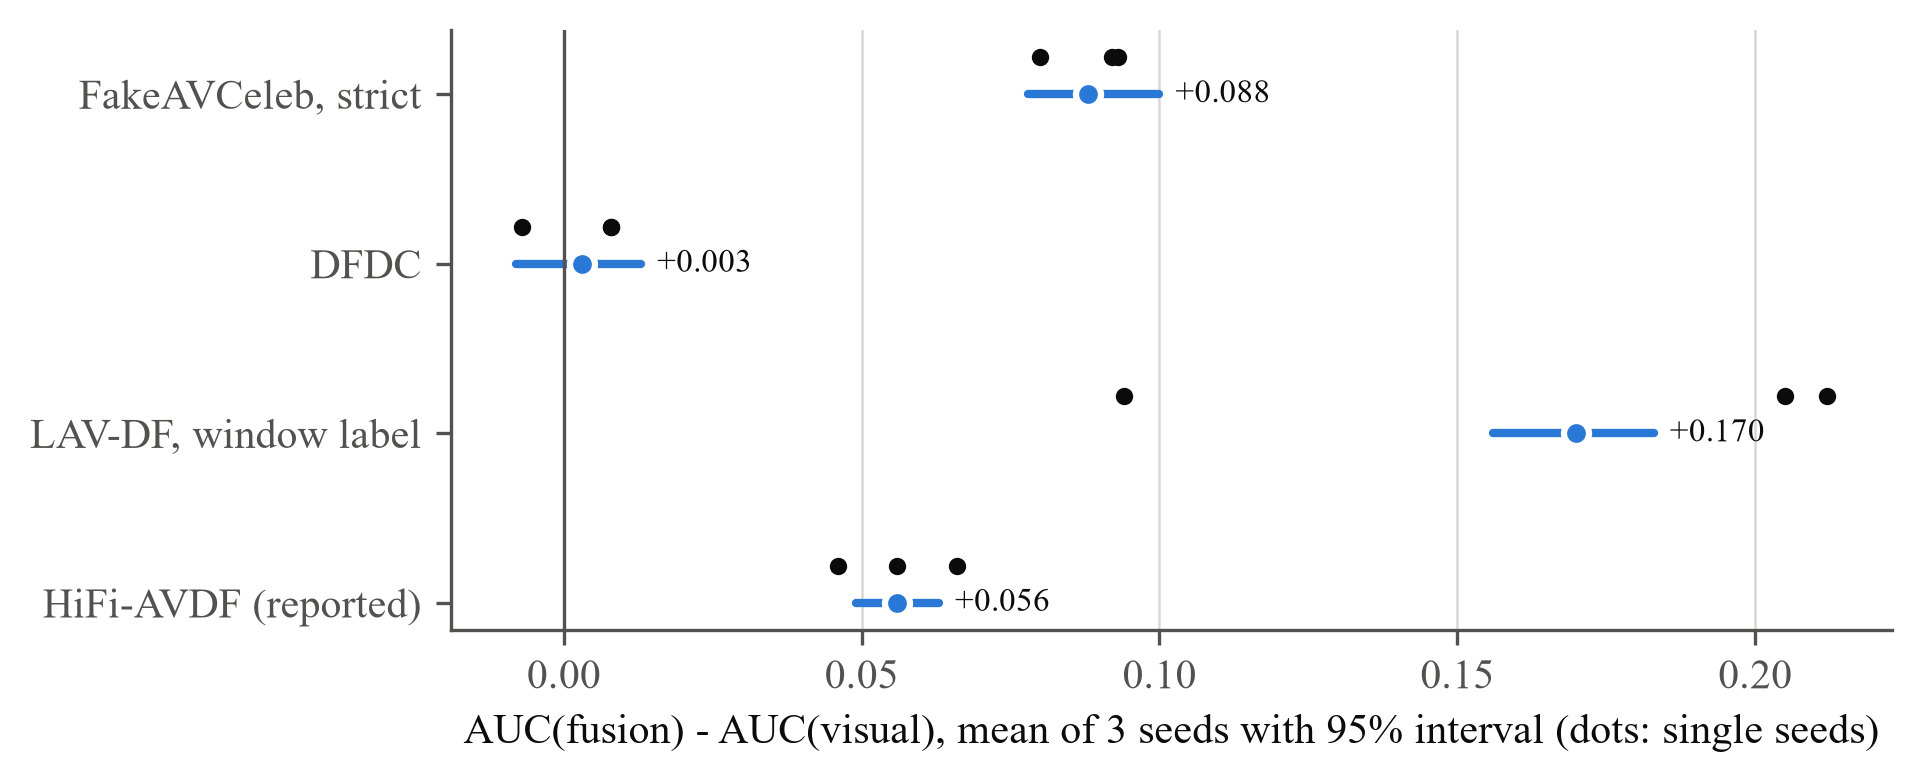
\includegraphics[width=0.85\textwidth,keepaspectratio]{fig_h2.png}
    \caption{Fusion minus visual-only ROC-AUC per target: the mean of three
    seeds with its 95\% interval, and each seed as a dot}
    \label{fig:h2}
\end{figure}

Table~\ref{tab:h2} and Figure~\ref{fig:h2} give the result. FakeAVCeleb and
LAV-DF survive Holm correction and DFDC does not, so H2 holds by its
preregistered rule. The seed-17
fusion weights on the standardized logits are {{h2.weights.seed17.visual}}
(visual), {{h2.weights.seed17.audio}} (audio) and {{h2.weights.seed17.sync}}
(sync).

\begin{table}[htbp]
    \centering
    \caption{ROC-AUC of each path on the clip label, over the clips H2
    compares: lowest and highest of three seeds}
    \label{tab:h2levels}
    \begin{tabular}{lllll}
        \toprule
        Target & Visual & Audio & Sync & Fusion \\
        \midrule
        FakeAVCeleb, strict & {{h2.test-identity-strict.auc.visual.min}}, {{h2.test-identity-strict.auc.visual.max}} & {{h2.test-identity-strict.auc.audio.min}}, {{h2.test-identity-strict.auc.audio.max}} & {{h2.test-identity-strict.auc.sync.min}}, {{h2.test-identity-strict.auc.sync.max}} & {{h2.test-identity-strict.auc.fusion.min}}, {{h2.test-identity-strict.auc.fusion.max}} \\
        DFDC & {{h2.dfdc.auc.visual.min}}, {{h2.dfdc.auc.visual.max}} & {{h2.dfdc.auc.audio.min}}, {{h2.dfdc.auc.audio.max}} & {{h2.dfdc.auc.sync.min}}, {{h2.dfdc.auc.sync.max}} & {{h2.dfdc.auc.fusion.min}}, {{h2.dfdc.auc.fusion.max}} \\
        LAV-DF, window & {{h2.lavdf-window.auc.visual.min}}, {{h2.lavdf-window.auc.visual.max}} & {{h2.lavdf-window.auc.audio.min}}, {{h2.lavdf-window.auc.audio.max}} & {{h2.lavdf-window.auc.sync.min}}, {{h2.lavdf-window.auc.sync.max}} & {{h2.lavdf-window.auc.fusion.min}}, {{h2.lavdf-window.auc.fusion.max}} \\
        \midrule
        HiFi-AVDF (reported) & {{h2.hifiavdf.auc.visual.min}}, {{h2.hifiavdf.auc.visual.max}} & {{h2.hifiavdf.auc.audio.min}}, {{h2.hifiavdf.auc.audio.max}} & {{h2.hifiavdf.auc.sync.min}}, {{h2.hifiavdf.auc.sync.max}} & {{h2.hifiavdf.auc.fusion.min}}, {{h2.hifiavdf.auc.fusion.max}} \\
        \bottomrule
    \end{tabular}
\end{table}

The result is weaker than the verdict suggests.
Two checks, run after the verdict and so exploratory, find that no target
shows fusion improving on fakes the visual path can see
(Table~\ref{tab:h2levels}).

\textbf{FakeAVCeleb.} The whole gain comes from the cloned-voice clips. The
visual path scores {{visual.test-identity-strict.seed17.auc}} (seed 17) on its
own video label but at most {{h2.test-identity-strict.auc.visual.max}} on the
clip label, where a clip with real video and a cloned voice counts as fake.
The visual path was trained never to flag those clips. Without them, the gain
falls from {{h2.test-identity-strict.estimate}} to between
{{h2.test-identity-strict.without_cloned_voice.min}} and
{{h2.test-identity-strict.without_cloned_voice.max}} per seed.

\textbf{LAV-DF.} The visual path ranks every fake type below the original real files
(AUC {{visual.lavdf-test.type.min}} to {{visual.lavdf-test.type.max}}),
including clips whose video was never edited
({{visual.lavdf-test.type.RealVideo-FakeAudio.min}} to
{{visual.lavdf-test.type.RealVideo-FakeAudio.max}}). A path that reacted to
face edits would score those near 0.5. So it reacts to some difference
between LAV-DF's real and fake files that is not the edit, and reads it
backwards. What that difference is, we do not know. The file-cue audit reads
metadata and cannot see it. Amendment A13 (exploratory) measured six
statistics of the face frames the path sees: sharpness, high frequencies,
blockiness, brightness, contrast and motion. None explains it. Each separates
the two groups at AUC {{a13.lavdf.auc_min}} to {{a13.lavdf.auc_max}}, and all
six together reach {{a13.lavdf.all_six}}, against the path's
{{a13.lavdf.visual}}. Its pooled AUC in Table~\ref{tab:h2levels} is higher,
though still below chance, because the window label counts as real the clips
cut from fake files with no edit in the window, and the path scores those as
low as the fakes. Fusion beats this reversed baseline but trails
the audio path and the sync path alone in every seed. Its weights were fit on
FakeAVCeleb, where the visual path is strong. Section~\ref{sec:a12} tests
whether that is to blame.

\textbf{DFDC.} Every clip in our subset has real audio. On the clip label the
audio path is near chance, the sync path is weak, and fusion adds nothing.

\textbf{HiFi-AVDF.} Reported outside the rule, it repeats the LAV-DF
pattern. Fusion gains {{h2.hifiavdf.estimate}} over a visual path near
chance, but trails the audio path alone in every seed.

\textbf{Stability.} The size of the gain depends on the seed, and so do the
weights: the audio weight is {{h2.weights.seed17.audio}},
{{h2.weights.seed29.audio}} and {{h2.weights.seed43.audio}} for seeds 17, 29
and 43.

So H2 shows that an audio path catches audio fakes a visual path cannot. It
does not show that fusion improves detection, or that it transfers to a new
corpus.

\section{Exploratory: A Fusion Fit on Other Corpora (A12)}
\label{sec:a12}

Amendment A12 was fixed after H2 was read and before this result existed. It
refits the same fusion, from the same logits, in two ways:
\begin{itemize}
    \item \textbf{Leave one out:} fit on the other two targets, then score the
    held-out one. This is a detector that never saw the target.
    \item \textbf{Upper bound:} a 5-fold cross-fit by identity on the target
    itself. It uses the target's labels, so it is not a detector. It shows
    whether the three paths hold any complementary information there.
\end{itemize}

\begin{table}[htbp]
    \centering
    \caption{A12 (exploratory): ROC-AUC on the clip label, mean of three seeds}
    \label{tab:a12}
    \begin{tabular}{lrrrrrr}
        \toprule
        Target & Visual & Audio & Sync & A8 & Leave one out & Upper bound \\
        \midrule
        DFDC & {{a12.dfdc.auc.visual}} & {{a12.dfdc.auc.audio}} & {{a12.dfdc.auc.sync}} & {{a12.dfdc.auc.a8}} & {{a12.dfdc.auc.leave_one_out}} & {{a12.dfdc.auc.upper_bound}} \\
        LAV-DF & {{a12.lavdf-window.auc.visual}} & {{a12.lavdf-window.auc.audio}} & {{a12.lavdf-window.auc.sync}} & {{a12.lavdf-window.auc.a8}} & {{a12.lavdf-window.auc.leave_one_out}} & {{a12.lavdf-window.auc.upper_bound}} \\
        HiFi-AVDF & {{a12.hifiavdf.auc.visual}} & {{a12.hifiavdf.auc.audio}} & {{a12.hifiavdf.auc.sync}} & {{a12.hifiavdf.auc.a8}} & {{a12.hifiavdf.auc.leave_one_out}} & {{a12.hifiavdf.auc.upper_bound}} \\
        \bottomrule
    \end{tabular}
\end{table}

\textbf{DFDC and HiFi-AVDF.} Even the upper bound does not beat the best
single path: {{a12.dfdc.upper_bound-minus-visual.estimate}}
[{{a12.dfdc.upper_bound-minus-visual.lower}},
{{a12.dfdc.upper_bound-minus-visual.upper}}] over the visual path on DFDC, and
{{a12.hifiavdf.upper_bound-minus-audio.estimate}}
[{{a12.hifiavdf.upper_bound-minus-audio.lower}},
{{a12.hifiavdf.upper_bound-minus-audio.upper}}] over the audio path on
HiFi-AVDF. No weighting of these paths helps there.

\textbf{LAV-DF.} The upper bound beats the audio path by
{{a12.lavdf-window.upper_bound-minus-audio.estimate}}
[{{a12.lavdf-window.upper_bound-minus-audio.lower}},
{{a12.lavdf-window.upper_bound-minus-audio.upper}}], so the paths do
complement each other a little. The leave-one-out fusion beats the A8 fusion
by {{a12.lavdf-window.leave_one_out-minus-a8.estimate}}, so weights from other
corpora help. It still trails the audio path
({{a12.lavdf-window.leave_one_out-minus-audio.estimate}}).

\textbf{Reading.} The best path changes with the corpus: visual on DFDC, audio
on the other two. So weights fit on some corpora point the wrong way on the
next. On DFDC the leave-one-out fusion falls to {{a12.dfdc.auc.leave_one_out}},
below chance. The FakeAVCeleb weights explain part of the loss on LAV-DF, but
the larger problem is that no fixed fusion of these paths transfers between
these corpora. A fusion that decides per clip which path to trust, and paths
trained on several corpora, are part of the full run
(Chapter~\ref{ch:future}).

\section{Exploratory: Stronger Frozen Backbones (A11)}
\label{sec:a11}

Published work reports that frozen CLIP ViT-L/14 features transfer far better
for faces, and XLS-R far better for speech, than the backbones P-001 uses. That
evidence comes from raw files, which carry the shortcuts this study measured.
Amendment A11 was fixed before either model existed. It trains both frozen on
the same cleaned data, splits and seeds, and compares each with its P-001 path
on the same clips.

\begin{table}[htbp]
    \centering
    \caption{A11 (exploratory): new path minus P-001 path, ROC-AUC on each
    path's own label, mean of three seeds with a 95\% identity-bootstrap
    interval}
    \label{tab:a11}
    \begin{tabular}{lll}
        \toprule
        Set & CLIP minus visual & XLS-R minus audio \\
        \midrule
        FakeAVCeleb, strict & {{a11.clip-vs-visual.test-identity-strict.estimate}} [{{a11.clip-vs-visual.test-identity-strict.lower}}, {{a11.clip-vs-visual.test-identity-strict.upper}}] & {{a11.xlsr-vs-audio.test-identity-strict.estimate}} [{{a11.xlsr-vs-audio.test-identity-strict.lower}}, {{a11.xlsr-vs-audio.test-identity-strict.upper}}] \\
        DFDC & {{a11.clip-vs-visual.dfdc.estimate}} [{{a11.clip-vs-visual.dfdc.lower}}, {{a11.clip-vs-visual.dfdc.upper}}] & one class \\
        LAV-DF test & {{a11.clip-vs-visual.lavdf-test.estimate}} [{{a11.clip-vs-visual.lavdf-test.lower}}, {{a11.clip-vs-visual.lavdf-test.upper}}] & {{a11.xlsr-vs-audio.lavdf-test.estimate}} [{{a11.xlsr-vs-audio.lavdf-test.lower}}, {{a11.xlsr-vs-audio.lavdf-test.upper}}] \\
        HiFi-AVDF & {{a11.clip-vs-visual.hifiavdf.estimate}} [{{a11.clip-vs-visual.hifiavdf.lower}}, {{a11.clip-vs-visual.hifiavdf.upper}}] & {{a11.xlsr-vs-audio.hifiavdf.estimate}} [{{a11.xlsr-vs-audio.hifiavdf.lower}}, {{a11.xlsr-vs-audio.hifiavdf.upper}}] \\
        \bottomrule
    \end{tabular}
\end{table}

\textbf{XLS-R.} It matches the P-001 audio path in-domain and is worse on
LAV-DF and HiFi-AVDF. On HiFi-AVDF it reaches
{{a11.xlsr-vs-audio.hifiavdf.auc_new}} against
{{a11.xlsr-vs-audio.hifiavdf.auc_old}}.

\textbf{CLIP.} It falls to {{a11.clip-vs-visual.test-identity-strict.auc_new}}
in-domain and to {{a11.clip-vs-visual.hifiavdf.auc_new}} on HiFi-AVDF. Its one
gain, on LAV-DF, takes it to {{a11.clip-vs-visual.lavdf-test.auc_new}}: near
chance, where the P-001 visual path is inverted
({{a11.clip-vs-visual.lavdf-test.auc_old}}). So CLIP does not read the
difference between LAV-DF's real and fake files that inverts the P-001 path,
but it does not detect LAV-DF's fakes either.

\textbf{Reading.} Our recipe differs from the published ones: no LayerNorm
tuning for CLIP, and no weighted sum of XLS-R layers. A published recipe might
do better. Under ours, the advantage measured on raw files does not survive the
shortcut control.

\section{Exploratory: Five Gaps Checked (A15 to A19)}
\label{sec:overnight}

Five further checks were fixed as dated amendments before their results
existed, to close gaps this report names. None changes a verdict.

\subsection{The sync mechanism (A16)}

On all {{a16.clips}} real FakeAVCeleb test clips we kept the lips at 0 to 2~s
and moved only the audio, then scored the window with the frozen sync heads
(Table~\ref{tab:a16}).

\begin{table}[htbp]
    \centering
    \caption{A16 (exploratory): the misfit of moved audio against the original window, mean of three seeds with a 95\% identity-bootstrap interval}
    \label{tab:a16}
    \begin{tabular}{lll}
        \toprule
        \textbf{Audio} & \textbf{AUC [95\%]} & \textbf{Clips whose misfit rose} \\
        \midrule
        1 frame later (0.04 s) & {{a16.shift004.auc}} [{{a16.shift004.low}}, {{a16.shift004.high}}] & {{a16.shift004.rising.min}} to {{a16.shift004.rising.max}} \\
        2 frames later (0.08 s) & {{a16.shift008.auc}} [{{a16.shift008.low}}, {{a16.shift008.high}}] & {{a16.shift008.rising.min}} to {{a16.shift008.rising.max}} \\
        0.20 s later & {{a16.shift020.auc}} [{{a16.shift020.low}}, {{a16.shift020.high}}] & {{a16.shift020.rising.min}} to {{a16.shift020.rising.max}} \\
        0.40 s later & {{a16.shift040.auc}} [{{a16.shift040.low}}, {{a16.shift040.high}}] & {{a16.shift040.rising.min}} to {{a16.shift040.rising.max}} \\
        0.80 s later & {{a16.shift080.auc}} [{{a16.shift080.low}}, {{a16.shift080.high}}] & {{a16.shift080.rising.min}} to {{a16.shift080.rising.max}} \\
        Another person's audio & {{a16.swap.auc}} [{{a16.swap.low}}, {{a16.swap.high}}] & {{a16.swap.rising.min}} to {{a16.swap.rising.max}} \\
        \bottomrule
    \end{tabular}
\end{table}

The score moves with the mechanism, which passes the rule fixed in A16. Shifts
of one and two frames are smaller than any the head saw in training, and they
still raise the misfit, though far less. The larger shifts and the swap
resemble the training negatives, so they confirm the trained objective on
people the head never saw.

\subsection{Which stream was faked, one direction (A15)}

H3 asks whether a model can say which stream was faked, in both directions
between FakeAVCeleb and LAV-DF. The reverse direction needs models trained on
LAV-DF, so H3 has still not run. A15 runs FakeAVCeleb to LAV-DF. The visual
and audio paths act as video-fake and audio-fake heads at their FakeAVCeleb
thresholds. The baseline marks both streams fake whenever the clip is fake.

The heads reach a macro-F1 of {{a15.window.heads.min}} to
{{a15.window.heads.max}} under the window label, against
{{a15.window.baseline}} for the baseline: a difference of
{{a15.window.estimate}} [{{a15.window.lower}}, {{a15.window.upper}}]. The
direction does not transfer. The video head is worse than guessing: its
precision ({{a15.window.video.seed17.precision}} at seed 17) is below the
share of clips whose video was edited. The audio head is precise when it fires
but recalls only {{a15.window.audio.seed43.recall}} to
{{a15.window.audio.seed17.recall}} of audio fakes at seeds 43 and 17. Its
ranking is fair (Chapter~\ref{ch:h2}), so the loss is in the threshold carried
over from FakeAVCeleb, as with the sync path in H4.

\subsection{Speaker overlap (A17)}

VoxCeleb2's dev and test speaker lists, checked against the published split,
place all {{a17.sources.dev}} FakeAVCeleb source identities in VoxCeleb2 dev
and none in test. AV-HuBERT pretrained on the English part of VoxCeleb2 dev,
so every FakeAVCeleb speaker may have been heard by the frozen encoder. No
unseen speaker exists in this corpus, so the effect cannot be measured here.
LAV-DF is also built from VoxCeleb2 but has no speaker ids.

\subsection{H1 with a fixed bitrate (A18)}

Video bitrate was the leading cue left after cleaning (Chapter~\ref{ch:protocol}).
A18 re-encoded all of FakeAVCeleb at a constant 160~kb/s, the median of the v4
copies, instead of a constant quality, and audited it again. The clip-label
ceiling falls only from {{audit.fakeavceleb.neutral.clip}} to
{{audit.fakeavceleb.cbr.clip}}, still above the bar of 0.60. The video-label
ceiling falls from {{audit.fakeavceleb.neutral.video}} to
{{audit.fakeavceleb.cbr.video}}, but the audio-label ceiling rises from
{{audit.fakeavceleb.neutral.audio}} to {{audit.fakeavceleb.cbr.audio}}. The
encoder overshoots its target by a few percent on busier content, and that
overshoot still follows the label; trailing silence and loudness after AAC
encoding remain. A fixed bitrate is not enough to meet H1.

\subsection{A published method on our protocol (A19)}

AVH-Align~\cite{smeu2025} is the closest published method. Its released
weights need features from a fine-tuned AV-HuBERT Large checkpoint that is not
available to us, so the published system was not run. Instead we retrained its
head, loss and score, changed only in input width, on the same real windows and
frozen features as our sync path (Table~\ref{tab:a19}).

\begin{table}[htbp]
    \centering
    \caption{A19 (exploratory): AVH-Align's method against the P-001 sync path on the same clips, mean of three seeds with 95\% identity-bootstrap intervals}
    \label{tab:a19}
    \begin{tabular}{lrll}
        \toprule
        \textbf{Set} & \textbf{Clips} & \textbf{AVH-Align [95\%]} & \textbf{Minus sync path [95\%]} \\
        \midrule
        FakeAVCeleb test & {{a19.test.clips|int}} & {{a19.test.auc}} [{{a19.test.low}}, {{a19.test.high}}] & {{a19.test.minus_sync.estimate}} [{{a19.test.minus_sync.lower}}, {{a19.test.minus_sync.upper}}] \\
        FakeAVCeleb, strict & {{a19.test-identity-strict.clips|int}} & {{a19.test-identity-strict.auc}} [{{a19.test-identity-strict.low}}, {{a19.test-identity-strict.high}}] & {{a19.test-identity-strict.minus_sync.estimate}} [{{a19.test-identity-strict.minus_sync.lower}}, {{a19.test-identity-strict.minus_sync.upper}}] \\
        LAV-DF, file label & {{a19.lavdf-test.clips|int}} & {{a19.lavdf-test.auc}} [{{a19.lavdf-test.low}}, {{a19.lavdf-test.high}}] & {{a19.lavdf-test.minus_sync.estimate}} [{{a19.lavdf-test.minus_sync.lower}}, {{a19.lavdf-test.minus_sync.upper}}] \\
        LAV-DF, window label & {{a19.lavdf-window.clips|int}} & {{a19.lavdf-window.auc}} [{{a19.lavdf-window.low}}, {{a19.lavdf-window.high}}] & {{a19.lavdf-window.minus_sync.estimate}} [{{a19.lavdf-window.minus_sync.lower}}, {{a19.lavdf-window.minus_sync.upper}}] \\
        DFDC & {{a19.dfdc.clips|int}} & {{a19.dfdc.auc}} [{{a19.dfdc.low}}, {{a19.dfdc.high}}] & {{a19.dfdc.minus_sync.estimate}} [{{a19.dfdc.minus_sync.lower}}, {{a19.dfdc.minus_sync.upper}}] \\
        HiFi-AVDF & {{a19.hifiavdf.clips|int}} & {{a19.hifiavdf.auc}} [{{a19.hifiavdf.low}}, {{a19.hifiavdf.high}}] & {{a19.hifiavdf.minus_sync.estimate}} [{{a19.hifiavdf.minus_sync.lower}}, {{a19.hifiavdf.minus_sync.upper}}] \\
        \bottomrule
    \end{tabular}
\end{table}

It does not beat the sync path on any set: it is worse on four and level on
two. On DFDC and HiFi-AVDF it is near chance. A different real-only alignment
head does not fix transfer. This compares two heads on our features and data,
not the published system, which was trained on 45,000 real AV-Deepfake1M
videos.

%
\chapter{Limitations and Future Scope}
\label{ch:future}

\section{Limitations}

\subsection{One training corpus}

Every model in this report learns from one corpus, FakeAVCeleb. It dates from
2021, has about 500 real videos, and its fakes are crude by today's standard.
The sync path learned from the real clips of about 350 speakers. A model that
has seen this little variety is expected to transfer poorly, so the
cross-corpus results describe how a detector trained this way transfers once
the shortcuts are gone. They do not show that every detector fails, or that
more and newer training data would not help. Testing that needs training on
several corpora with one held out at a time, which is the main protocol we
propose next (Section~\ref{sec:next}).

\subsection{H1 missed its preregistered bar}

The neutral FakeAVCeleb ceiling is {{audit.fakeavceleb.neutral.clip}}, against
a bar of 0.60. The main residual is video bitrate. Under constant-quality
encoding it follows image content, so it is partly a property of the
manipulated pixels. That explanation does not change the result. H1 failed as
written, and every result on the neutral copies carries that caveat.

\subsection{A residual audio-label cue}

The ceiling on the audio label stays at {{audit.fakeavceleb.neutral.audio}}.
It comes from millisecond differences at clip ends and from loudness after
AAC encoding. Any claim about which modality was faked must be read beside
this number. It also leaves room for the sync path's success on cloned voices
to come partly from audio properties (Chapter~\ref{ch:sync}).

Amendment A14 (exploratory) checked whether the audio path relies on those two
cues. With every clip's loudness levelled and 250~ms cut from each edge, its
AUC on the identity-strict test stays between
{{a14.test-identity-strict.perturbed_min}} and
{{a14.test-identity-strict.perturbed_max}} across the three seeds. So the
named cues do not drive the audio path. Cues the audit did not name are not
covered.

\subsection{Refusals}

The neutralizer refused {{neutral.fakeavceleb.refused|int}} short clips, all
generated speech and none real. Results on the neutral copies describe clips
with at least 3.00 s of sound. They say nothing about very short generated
clips.

\subsection{Parts of the study that have not run}

Two parts of the preregistered study are incomplete in this version, and the
secondary fusion model was dropped for the deadline window (amendment A8):

\begin{itemize}
    \item \textbf{Modality prediction (H3).} Only the direction from
    FakeAVCeleb to LAV-DF has run, as exploratory amendment A15, and it does
    not transfer. The reverse needs models trained on LAV-DF.
    \item \textbf{Baselines.} AVH-Align's method has run on our protocol
    (A19), but not its published system. HAVIC~\cite{havic} has not been
    run. HAVIC's released
    weights can be scored on HiFi-AVDF, DFDC and LAV-DF. They cannot be scored
    fairly on our FakeAVCeleb test, because HAVIC was fine-tuned on a random,
    ungrouped FakeAVCeleb split and has almost certainly seen our test
    identities.
\end{itemize}

\subsection{Speaker overlap with AV-HuBERT pretraining}

AV-HuBERT was pretrained on LRS3 and VoxCeleb2. Amendment A17 found every
FakeAVCeleb speaker in VoxCeleb2 dev, the part used for pretraining, and none
in VoxCeleb2 test. LAV-DF is also built from VoxCeleb2 but has no speaker ids.
Some of the sync path's signal may come from the encoder having heard these
speakers before. With no unseen speaker in FakeAVCeleb, its size cannot be
measured here.

\subsection{Too few real clips in DFDC for H4}

Our DFDC subset has {{audit.dfdc.raw.census.RealVideo-RealAudio.clips|int}}
real clips. H4 needs 200 for calibration and more to score. So H4 runs on
LAV-DF and HiFi-AVDF only.

\subsection{Other limits}

\begin{itemize}
    \item \textbf{Neutralization may remove real evidence.} Re-encoding can
    blur fine blending artifacts, and cutting edge silence can remove a real
    generator trace. We have not yet measured what neutralization costs a
    detector on a corpus where the codec does not follow the label.
    \item \textbf{The sync path alone misses face swaps.} By design it cannot
    catch a fake that keeps the original lips and voice.
\end{itemize}

\section{The Full-Run Plan}
\label{sec:next}

This report follows the short plan chosen for the submission deadline, three
days from 16 November 2026. The full study runs after the deadline, in this
order:

\begin{enumerate}
    \item Train on several corpora with one held out at a time
    (leave-one-corpus-out), so every test stays unseen while the models see
    more variety. This needs a new preregistration, P-002, because LAV-DF and
    DFDC would no longer be locked targets.
    \item Speed up the cache build for the visual and audio paths.
    \item Run the StreamFusion model, the secondary fusion, against the
    logistic fusion of H2.
    \item Train the reverse models on LAV-DF and run H3 in both directions.
    \item Run HAVIC, and AVH-Align's published system with fine-tuned
    AV-HuBERT Large features, on our protocol.
    \item Add AV-Deepfake1M and KoDF if access arrives. Both were requested,
    along with AV-Deepfake1M++ and DeepSpeak v2.
    \item Write the full paper.
\end{enumerate}

The results in this report stay valid in the full run. It reuses the same
frozen sync models, neutral copies and splits. When new results arrive, the
deliverables are rebuilt from the larger result file, so no result is copied
by hand.

One further check would close an open objection: measure the cost of
neutralization on LAV-DF, by training and testing on raw files, then on
neutral files, where the codec does not follow the label. The direct test of
the sync mechanism has run (A16).

%
\chapter{Conclusion}
\label{ch:conclusions}

We set out to measure how much of audio-visual deepfake benchmark accuracy
comes from how the files were made. On FakeAVCeleb, file metadata and audio
edges alone predict the label at {{audit.fakeavceleb.raw.clip}}. HiFi-AVDF, a
modern set of six commercial generators, reaches
{{audit.hifiavdf.raw.clip}} from export settings alone. LAV-DF leaks through
weak cues added together. DFDC barely leaks. A detector score on any of these
corpora means little until it is set beside the shortcut ceiling of the same
data.

Our first neutralizer put the shortcut back through hidden AAC padding. The final version brought the
FakeAVCeleb ceiling down to {{audit.fakeavceleb.neutral.clip}}. That missed the
bar we set in advance, and we report it as a miss. Cleaning also refused
{{neutral.fakeavceleb.refused|int}} short clips, all of them generated speech.

On those neutral copies, we trained a lip-sync detector that never saw a fake.
It reached a test AUC of {{sync.test.seed17.auc}}, {{sync.test.seed29.auc}}
and {{sync.test.seed43.auc}} at three seeds. All three sit above the ceiling of
the same data.
Its pattern across methods matches its mechanism. It catches cloned voices
best and plain face swaps least. Its weak point is false alarms at a carried-over
threshold, which Chapter~\ref{ch:crosscorpus} addresses with thresholds set
from real clips of each new domain.

On corpora it never saw, the detector stays above chance but falls far: its
AUC lies between {{sync.dfdc.seed17.auc}} and
{{sync.lavdf-window.seed29.auc}} on DFDC, LAV-DF and HiFi-AVDF. A threshold set
from 200 real clips of the new corpus brings false alarms on HiFi-AVDF to
{{h4.hifiavdf-seed43.conformal_real_only.fpr}} to
{{h4.hifiavdf-seed17.conformal_real_only.fpr}}, from
{{h4.hifiavdf-seed43.source_validation.fpr}} to
{{h4.hifiavdf-seed17.source_validation.fpr}}, but it then catches few fakes.

Fusing the visual, audio and sync paths passes its preregistered test
(Chapter~\ref{ch:h2}). The gain comes from fakes the visual path cannot see,
and on LAV-DF from a visual path that the files invert. No fixed fusion of these
paths transferred between corpora, and stronger frozen backbones did not
transfer better on the cleaned data.

The earlier phases of this project produced many strong numbers that did not
survive scrutiny. This version produces fewer numbers, and each one comes with
the data that could explain it away. The main lesson is a working habit: before
training a detector, measure what the files alone can do.

%
\appendix
\chapter{Reproducibility}
\label{app:repro}

\section{Commands}

Every result in Chapters~\ref{ch:audit} to~\ref{ch:sync} can be rebuilt with
the commands below, run from the repository root with the project's own Python
interpreter. Each command line is wrapped for the page.

\begin{enumerate}
    \item \textbf{Shortcut audit of the raw files.}\\
    {\small\ttfamily\raggedright .venv/Scripts/python.exe scripts/shortcut\_audit.py -{}-manifest data/manifests/fakeavceleb.csv -{}-dataset FakeAVCeleb -{}-output results/shortcut-audit/fakeavceleb\par}
    \item \textbf{Neutral copies and their manifest.}\\
    {\small\ttfamily\raggedright .venv/Scripts/python.exe scripts/neutralize\_dataset.py -{}-manifest data/manifests/fakeavceleb.csv -{}-dataset FakeAVCeleb -{}-output-root data/neutral -{}-manifest-out data/manifests/fakeavceleb-neutral.csv\par}
    \item \textbf{Identity-disjoint split.}\\
    {\small\ttfamily\raggedright .venv/Scripts/ddf.exe split build -{}-manifest data/manifests/fakeavceleb-neutral.csv -{}-output-dir runs/p001/split -{}-dataset FakeAVCeleb -{}-seed 17\par}
    \item \textbf{Frozen AV-HuBERT features,} two 2-second windows per clip at a 1-second step.\\
    {\small\ttfamily\raggedright .venv/Scripts/python.exe scripts/extract\_avhubert\_features.py -{}-manifest data/manifests/fakeavceleb-neutral.csv -{}-cuts data/manifests/fakeavceleb-neutral.cuts.csv -{}-windows 2 -{}-step 1 -{}-output runs/avhubert-fakeavceleb-neutral\par}
    \item \textbf{Train and score the sync path} at seeds 17, 29 and 43.\\
    {\small\ttfamily\raggedright .venv/Scripts/python.exe scripts/train\_sync\_path.py -{}-features runs/avhubert-fakeavceleb-neutral -{}-split-dir runs/p001/split -{}-output runs/p001/sync\par}
\end{enumerate}

The later stages run from driver scripts in \texttt{runs/}, the only files
tracked in that folder:

\begin{itemize}
    \item \texttt{runs/p001-2day.sh}: the cross-corpus and false-alarm steps
    of Chapter~\ref{ch:crosscorpus}. It neutralizes each target, extracts
    features, scores the frozen heads, evaluates them with receipts, runs
    \texttt{scripts/run\_h4.py}, and audits the neutral copies.
    \item \texttt{runs/p001-a10.sh}: the second face locator of amendment A10,
    and the rescoring that follows it.
    \item \texttt{scripts/run\_p001\_branches.sh}: the visual and audio paths.
    \item \texttt{runs/p001-h2.sh}: target caching and
    \texttt{scripts/run\_h2.py} for Chapter~\ref{ch:h2}.
    \item \texttt{runs/p001-a11.sh} and \texttt{runs/p001-a13-a14.sh}: the
    exploratory amendments A11, A13 and A14; \texttt{scripts/run\_a12.py}
    runs A12 from the H2 logits.
    \item \texttt{runs/p001-finalize.sh}: copies the outputs into
    \texttt{results/} and rebuilds every number, figure and deliverable.
\end{itemize}

\section{Results Layout}

\begin{itemize}
    \item \texttt{results/preregistration/} holds P-001 and its amendments.
    Each was committed before the run it governs.
    \item \texttt{results/shortcut-audit/<corpus>/} holds each audit:
    \texttt{summary.json} with the ceilings, single-cue AUCs and codec census,
    and \texttt{clips.csv} with every clip's measured cues. Neutral audits add
    \texttt{neutralize-summary.json}, which counts refusals per category, and
    \texttt{cuts.csv}, which records every cut.
    \item \texttt{results/p001-sync/} holds the sync path's metrics and
    per-clip predictions for each set and seed. It also holds the validation
    thresholds with the clip ids that chose them, the selection record in
    \texttt{training.json}, and the receipts.
    \item \texttt{results/p001-sync-targets/} and \texttt{results/p001-h4/}
    hold the cross-corpus scores and H4; the \texttt{-pre-a10} folders keep
    the versions from before amendment A10.
    \item \texttt{results/p001-branches/} and \texttt{results/p001-h2/} hold
    the visual and audio paths and the H2 fusion, and
    \texttt{results/p001-a11/} to \texttt{results/p001-a14/} the exploratory
    checks.
    \item Apart from its driver scripts, \texttt{runs/} is not tracked. It
    holds large intermediate files: neutral clips, features and checkpoints.
\end{itemize}

\section{Receipts}

Each receipted stage writes a JSON file with four parts: the exact command,
and SHA-256 hashes of the input files, the code files and the output files.
The tool \texttt{scripts/research\_artifacts.py} writes and checks them. A
stage whose receipt matches its current files is skipped on rerun. Feature
extraction and sync training ran before receipts existed, so those two stages
have none. Their outputs are committed with per-clip predictions, so every
metric can be recomputed from them.

\section{How Numbers Enter This Report}

No number in this report was typed by hand. The script
\texttt{scripts/build\_numbers.py} collects every reported value from the
committed result files into \texttt{results/numbers.json}, each with its
source file. The script \texttt{scripts/fill\_numbers.py} then fills the
placeholders in this report's source. A placeholder whose value is missing
stops the build, so the report can never ship with a gap or a stale value.

%
\addcontentsline{toc}{chapter}{Bibliography}
\bibliographystyle{IEEEtran}
\bibliography{references}

\end{document}
